%\documentclass{sig-alternate-10pt}
\documentclass[10pt]{sigalternate052015}

\usepackage{amsmath}
\usepackage{amssymb}
\usepackage{xcolor}
\usepackage{url}
\usepackage{times}
\usepackage{xspace}
\usepackage{listings}
\usepackage{code}
\usepackage{algorithm}
\usepackage[noend]{algpseudocode}
\usepackage{tikz}
\usetikzlibrary{arrows,automata,positioning}
\let\proof\relax
\let\endproof\relax
\usepackage{amsthm}
\usepackage{subcaption}
%\usepackage{geometry}

\usepackage{balance}


\definecolor{princetonorange}{RGB}{255,143,0}
\definecolor{tmlblue}{RGB}{0,58,120}  % tmlblue == Toronto Maple Leafs Blue!

\newcommand{\todo}[1]{\textcolor{red}{[TODO: #1]}}
\newcommand{\ratul}[1]{\textcolor{blue}{[ratul: #1]}}
\newcommand{\ryan}[1]{\textcolor{green}{[ryan: #1]}}
\newcommand{\dpw}[1]{\textcolor{tmlblue}{[dpw: #1]}}
\newcommand{\todd}[1]{\textcolor{princetonorange}{[todd: #1]}}

\newcommand{\EG}{\emph{e.g.}}
\newcommand{\IE}{\emph{i.e.}}
\newcommand{\ETC}{\emph{etc.}}
\newcommand{\ETAL}{\emph{et al.}}

\newcommand{\sysname}{{\small \sf Propane}\xspace}

\newcommand{\para}[1]{\paragraph*{\textbf{#1}}}

\newcommand{\set}[1]{\ensuremath{\{ #1 \} }}
\newcommand{\abs}[1]{\ensuremath{ \lvert #1 \rvert }}

\newcommand{\CD}[1]{\texttt{\small #1}}  % code font
\newcommand{\KW}[1]{\texttt{\small\bfseries{#1}}}
%\newcommand{\KW}[1]{\texttt{#1}}
\newcommand{\True}{\CD{true}}
\newcommand{\Define}{\KW{define}}
\newcommand{\Prefer}{\texttt{>>}}
\newcommand{\Path}{\texttt{=>}}
\newcommand{\Link}{\texttt{->}}
\newcommand{\Agg}{\KW{agg}}
\newcommand{\Any}{\KW{any}}
\newcommand{\None}{\KW{drop}}
\newcommand{\In}{\KW{in}}
\newcommand{\Out}{\KW{out}}
\newcommand{\AND}{\texttt{\&}}
\newcommand{\OR}{\texttt{|}}
\newcommand{\NOT}{\texttt{!}}
\newcommand{\Intersect}{\ensuremath{\cap}}
\newcommand{\Union}{\ensuremath{\cup}}

\newcommand{\Exit}{\KW{exit}}
\newcommand{\End}{\KW{end}}
\newcommand{\Start}{\KW{start}}
\newcommand{\Enter}{\KW{enter}}
\newcommand{\Later}{\KW{later}}
\newcommand{\Before}{\KW{before}}
\newcommand{\Internal}{\KW{internal}}
\newcommand{\Never}{\KW{never}}
\newcommand{\Only}{\KW{only}}
\newcommand{\Through}{\KW{through}}
\newcommand{\LinkKW}{\KW{link}}
\newcommand{\PathKW}{\KW{path}}
\newcommand{\Novalley}{\KW{novalley}}

%\let\Url\url
%\renewcommand*{\LaTeX}{\oldLaTeX\space}
\renewcommand{\path}[2]{ #1 \mapsto \ensuremath{#2} }



\begin{document}

\setcopyright{acmcopyright}
\conferenceinfo{SIGCOMM '16}{August 22--26, 2016, Florianopolis, Brazil}





\special{papersize=8.5in,11in}
\setlength{\pdfpageheight}{\paperheight}
\setlength{\pdfpagewidth}{\paperwidth}

\title{Don't Mind the Gap:  Bridging Network-wide Objectives and Device-level Configurations}

%\author{Paper \#324, 14 pages}


\author{%
Ryan Beckett\\
  \affaddr{Princeton University}
  %\\
  %\email{rbeckett@princeton.edu}
\and
Ratul Mahajan\\
  \affaddr{Microsoft Research}
  %\\
  %\email{ratul@microsoft.com}
\and
Todd Millstein\\
  \affaddr{University of California, Los Angeles}
  %\\
  %\email{todd@cs.ucla.edu}
\and
Jitu Padhye\\
  \affaddr{Microsoft Research}
  %\\
  %\email{padhye@microsoft.com}
\and
David Walker\\
  \affaddr{Princeton University}
  %\\
  %\email{dpw@princeton.edu}
}

\maketitle



%=====================================================
%
%
%  **Abstract**
%
%
%=====================================================

%\textbf{Abstract---}
%% Networks are notoriously difficult to configure correctly.
%% Operators typically rely on local configuration of individual devices running
%% distributed control plane protocols to achieve network-wide objectives.
%% Managing implicit dependencies between device configurations and properly accounting for failures makes
%% a network operator's work particularly difficult.
%% %
%% %The recent move towards software-defined networking has been motivated, in part,
%% %by the simplicity of the centralized model, where a controller directly manages
%% %individual devices rather than letting them manage themselves. However distributed
%% %protocols have many important advantages in scalability,
%% %latency and fault tolerance over the completely centralized approach.
%% %
%% In this paper, we describe a new system -- \sysname, which allows an operator to specify a high-level,
%% centralized routing policy declaratively, but then to compile it to a purely distributed
%% implementation, which uses the BGP routing protocol to run on existing, commodity hardware.
%% %
%% Propane allows operators to describe the types of paths traffic may (or may not) take
%% through the network, as well as relative preferences (or backups) between paths.
%% %
%% Network policies compiled with \sysname are guaranteed to implement the correct routing policy regardless of the number of failures, if possible.  If this is not possible, the compiler notifies the user at compile time rather than as the network is in
%% operation.
%% %
%% %\sysname also takes the centralized model one step further by unifying inter and intra-domain routing. Operators can specify routing policy for an autonomous system by programming against the abstraction that they can control any route in the wider internet.
%% %
%% We have implemented a compiler for \sysname and evaluated it against several real-world configurations for datacenters and core backbone networks. We demonstrate the \sysname compiler can scale to
%% topologies with thousands of routers.
%
%\begin{abstract}
%Traditional network operators have a difficult job: They are charged
%with achieving network-wide objectives, but they must do so by
%managing many individual, separate devices, each of which is running a
%complex distributed control plane protocol.  Bridging the gap between
%high-level objectives and low-level mechanisms manually is a challenging and
%error-prone task.
%%
%In this paper, we describe our preliminary efforts to design and
%implement a new language called Propane, which simplifies the task of
%network management by allowing operators to specify their objectives
%using end-to-end forwarding paths rather than device-by-device
%configurations.  A compiler rather than a human bridges the gap
%between high-level goals and the low-level mechanisms.  More
%specifically, Propane allows operators to describe and rank the sets
%of paths that traffic may follow.  Such paths stretch from external
%ASes, through the user's network, and possibly onward again to other
%ASes.  The Propane compiler analyzes these user specifications and
%then compiles them to a collection of BGP configurations, so they may
%exploit existing distributed fault tolerance mechanisms and
%execute on existing commodity hardware.  During the compilation
%process, it automatically synthesizes per-device import and export
%filters, local preferences, MED attributes, and community tags.  An
%important feature of the language is that whenever possible, compiled
%configurations are guaranteed to implement the correct routing policy,
%regardless of the number of failures.  If correct compilation is
%impossible, the compiler notifies the user at compile time rather than
%waiting until the system is in operation and failures have occurred.
%To date, we have used the language and compiler to experiment with
%several real-world configurations for datacenters and core backbone
%networks.  We demonstrate our prototype compiler can scale to
%topologies with thousands of routers.
%\end{abstract}

%\textbf{Abstract---}
%We develop a system called \sysname to help network operators with a challenging and error prone task: bridging the gap between network-wide routing objectives and low-level configurations of devices that run complex distributed protocols.
%%
%\sysname allows operators to specify their objectives naturally, describing high-level constraints and preferences on the types of paths that traffic should take through their network or other networks.
%%using ranked sets of paths which may be partial or end-to-end and may also refer to other networks.
%%
%Our compiler automatically translates these specifications to a collection of BGP router configurations.
%% that can execute on existing commodity hardware.
%%
%We introduce data structures and algorithms that guarantee that the compiled, distributed configurations correctly implement the routing policy under all possible combinations of failures.
%%
%We use \sysname to specify and compile the configurations of real
%datacenter and backbone networks.  We show that, despite its strong guarantees, it scales to topologies with hundreds to thousands of routers.

\textbf{Abstract---}
We develop \sysname, a language and a compiler to help network operators with a challenging, error-prone task: bridging the gap between network-wide routing objectives and low-level configurations of devices that run complex, distributed protocols.
%
The language allows operators to specify their objectives naturally, using high-level constraints and ordered preferences on paths that traffic should take.
%through their network or other networks.
%using ranked sets of paths which may be partial or end-to-end and may also refer to other networks.
%
The compiler automatically translates these specifications to router-level BGP configurations, using a novel data structure that compactly encodes the flow of routing information along policy-compliant paths.
%It uses We introduce data structures and algorithms that
It guarantees that the compiled configurations correctly implement the specified policy under all possible combinations of failures.
%
We use \sysname for datacenter and backbone networks of a large cloud provider. We find that our language can effectively express their policies and, despite its strong guarantees, our compiler scales to topologies with hundreds or thousands of routers.



%=====================================================
%
%
%  **Keywords**
%
%
%=====================================================

%\category{CR-number}{subcategory}{third-level}

\begin{CCSXML}
<ccs2012>
<concept>
<concept_id>10003033.10003068.10003073.10003075</concept_id>
<concept_desc>Networks~Network control algorithms</concept_desc>
<concept_significance>300</concept_significance>
</concept>
<concept>
<concept_id>10011007.10011006.10011050.10011017</concept_id>
<concept_desc>Software and its engineering~Domain specific languages</concept_desc>
<concept_significance>300</concept_significance>
</concept>
</ccs2012>
\end{CCSXML}

\ccsdesc[300]{Networks~Network control algorithms}
\ccsdesc[300]{Software and its engineering~Domain specific languages}

\printccsdesc

\keywords{Propane; Domain-specific Language; BGP; Synthesis; Compilation; Fault tolerance}

%% general terms are not compulsory anymore,
%% you may leave them out
%\terms Network Programming Language, Distributed Program Synthesis
%\keywords Propane Language, BGP, Synthesis, Compilation

%=====================================================
%
%
%  **Introduction**
%
%
%=====================================================


\section{Introduction}
\label{sec:introduction}

It is well known that configuring networks is error
prone and such errors can lead to disruptive
downtimes~\cite{mahajan+:bgp-misconfiguration,feamster+:rcc,batfish,dc-failure-study}.
For instance, a recent misconfiguration led to an hour-long, nation-wide outage for Time Warner's backbone network~\cite{time-warner}; and a major BGP-related incident makes international news every few months~\cite{bgpmon}.

%For instance, in the context of BGP, Mahajan~~\cite{mahajan+:bgp-misconfiguration}
%estimated that 200-1200 prefixes suffered from
%misconfiguration each day and that close to 3 in 4 of all
%new prefix advertisements were the result of misconfiguration.
%Moreover, these misconfigurations sometimes cause significant network downtime for
%individual networks~\cite{time-warner} or even broader internet connectivity problems~\cite{routing-instability,mahajan+:bgp-misconfiguration}.
%\dpw{Note that \cite{time-warner} and I am not sure about the specifics of the problem there
%or what exactly was misconfigured.  It is also unclear if our language really helps with the
%``broader internet connectivity problems'' however, I thought that adding some specific examples
%would help make the intro more compelling.  Feel free to rewrite.}

%One reason for network configuration being onerous is that device configuration languages are low-level and several configuration elements must be kept consistent (e.g., interface addresses) for the device to behave as intended.

A fundamental reason for the prevalence of misconfigurations is the
semantic mismatch between the intended high-level
policies and the low-level configurations.
Many policies involve network-wide properties---prefer a certain neighbor,
never announce a particular destination externally,
use a particular path only if another fails---but configurations describe the behavior of
individual devices.
%
Operators must manually decompose network-wide policy into
device behaviors, such that policy-compliant behavior results from the distributed interactions of
these devices.
%
Policy-compliance must be ensured not only under normal
circumstances but also during failures.  The need to reason
about all possible failures exacerbates the challenge
for network operators.  As a result, configurations that work
correctly in failure-free environments have nonetheless been found to violate key
network-wide properties when failures occur~\cite{batfish}.

To reduce configuration errors, operators are increasingly adopting an
approach in which common tasks are captured as parameterized templates~\cite{hatch,thwack}.
%
%More powerful still are systems like
%ConfigAssure~\cite{narain:lisa05,narain+:configassure}, which use SAT solving
%and model finding tools to fill in parameters in configurations while
%ensuring key correctness constraints are satisfied.
%One step further, systems like
%ConfigAssure~\cite{narain:lisa05,narain+:configassure} use SAT solving
%and model finding tools to correctly and consistently fill in some parameters.
%
While templates help ensure certain kinds of consistency across devices,
they do not provide fundamentally different abstractions from existing configuration languages
or bridge the semantic divide between network-wide policies and device-level configuration.
%They do not provide fundamentally different abstractions
%from existing configuration languages and
Thus, they still require operators to
manually decompose policies into device behaviors.

As a complementary approach, configuration analysis tools can help reduce misconfigurations by checking if low-level configurations match high-level policy~\cite{batfish,feamster+:rcc}. However, such tools too cannot help operators with the challenging task of generating configurations in the first place.

%Further, today's tools cannot verify correctness under concrete failure scenarios, rather than under all possible failures.

Software-defined networking (SDN) and its abstractions
are, in part, the research
community's response to the difficulty of maintaining policy
compliance through distributed device interactions~\cite{ethane}.
Instead of organizing networks around a distributed
collection of devices that compute forwarding tables through
mutual interactions, the devices are told how to
forward packets by a centralized controller. The controller is responsible for ensuring that the
paths taken are compliant with operator specifications.
%Researchers
%have developed increasingly sophisticated languages that let operators
%specify desirable network paths~\cite{x,y,z} which are then translated
%to forwarding tables at runtime.

The centralized control planes of SDN, however, are not a panacea.
First, while many SDN programming systems~\cite{sdn-languages} provide effective \emph{intra}-domain routing
abstractions, letting users specify paths within their network,
they fail to provide a coherent means to specify \emph{inter}-domain routes.
Second, centralized control planes
require careful design and engineering to be robust to failures---one must ensure that all devices can communicate with the controller at all times, even under arbitrary failure combinations. Even ignoring failures, it is necessary for the control system to
scale to meet the demands of large or geographically-distributed networks,
and to react quickly
to environmental changes. For this challenge, researchers are exploring
multi-controller systems with interacting controllers, thus bringing back distributed
control planes~\cite{mccauley2013extending,onos} and their current programming difficulties.
%However, academic
%language design and implementation efforts have not kept pace.  For instance, work on many
%experimental SDN languages~\cite{frenetic,flowlog,vericon,merlin,netkat,kinetic,pga} has not yet shown how to implement fault tolerant
%multi-controller systems that support their high-level abstractions efficiently.

Hence, in this paper, we have two central goals:
\begin{enumerate}
\item Design a new, high-level language with natural abstractions
for expressing intra-domain routing, inter-domain
routing and routing alternatives in case of failures.
\item Define algorithms for compiling these specifications into
configurations for devices running standard
distributed control plane algorithms, while ensuring correct behavior
independent of the number of faults.
\end{enumerate}

To achieve the first goal, we borrow the idea of using regular
expressions to specify network paths from
recent high-level SDN languages such as FatTire~\cite{fattire},
Merlin~\cite{foster:merlin}, and
NetKAT~\cite{netkat}.  However, our design also contains several key
departures from existing languages.  The most important one is semantic:  the paths specified
can extend from outside the operator's network to inside
the network, across several devices internally, and then out again. This design
choice allows users to specify preferences about both external and internal
routes in the exact same way.
In addition, we augment the algebra
of regular expressions to support a notion of {\em preferences} and provide a semantics in terms of sets of ranked paths. The preferences indicate fail-over behaviors:  among all specified paths that are still available,
the system guarantees that the distributed implementation will always use the highest-ranked ones.
Although we target a distributed implementation, the language is more general and could potentially be used in an SDN context.

%We also support network operators by defining a
%set of common abbreviations for entering, leaving, and traversing
%the user network and we provide abstractions for managing common features %of
%control plane algorithms such as route aggregation.  Operators use familiar logical operations
%to build routes in a modular and compositional manner from these
%primitives.  Our abbreviations are translated in to our regular-expression-based
%intermediate representation and compiled from there.

To achieve the second goal, we develop program analysis and compilation
algorithms that translate the regular policies to a graph-based
intermediate representation and from there to per-device BGP configurations, which include various filters and preferences that govern BGP behavior.
%import and export filters, local preferences, MED attributes, and community tags.
We target BGP for pragmatic reasons:
it is a highly flexible routing protocol,
it is an industry standard,
and many networks use it internally as well as externally.
Despite the advent of SDN, many networks will continue to
use BGP for the foreseeable future due to existing infrastructure investments, the difficulty of transitioning to SDN, and the scalability and fault-tolerance advantages of a distributed
control plane.

The BGP configurations produced by our compiler are
guaranteed to be policy-compliant in the face of
{\em arbitrary} failures.\footnote{We assume that BGP is the only routing protocol running in the network or the other protocols are correctly configured and do not have adverse interactions with BGP~\cite{igp-correctness1,igp-correctness2}.} This guarantee does not mean that the implementation is always
able to send traffic to its ultimate destination
(\EG, in the case of a network partition), but rather that it always respects the
centralized policy, which may include dropping traffic when there is no route.
%
In this way, we provide network operators
with a strong guarantee that is otherwise impossible to achieve
today.
However, some policies simply cannot be implemented correctly in BGP in
 the presence of arbitrary failures.  We develop new
algorithms to detect such policies
and report our findings to the operators, so they may fix the policy
specification at compile time rather than experience undesirable
behavior after the configurations are deployed.
%We also analyze route aggregation to detect the possibility of failure-induced black-holes.

%These algorithms differ from
%standard BGP analysis algorithms~\cite{feamster:rcc,batfish} because they operate on
%our graph-based intermediate representation, which operates at a higher level
%of abstraction than raw BGP configurations (and which has the pleasant effect of simplifying our
%task).

We have implemented our language and compiler in a system called \sysname. To evaluate it, we use it to specify real policies of datacenter and backbone networks.
% and compared these specifications with existing configurations.
We find that our language expresses such policies easily, and that the compiler scales to topologies with hundreds to thousands of routers, compiling in under 9 minutes in all cases.

%measured the performance of our compiler, demonstrating that our compilation
%algorithms scale to topologies with several thousand routers.
%
%\dpw{The following could be cut for space.}
%In the remainder of the paper, we review BGP (Section~\ref{sec:background}---readers
%familiar with BGP may skip this section),
%further motivate the need for new languages
%for programming distributed control planes (Section \ref{sec:motivation}),
%introduce \sysname{} by example (Section \ref{sec:propane}),
%explain our compiler algorithms (Section \ref{sec:compilation}),
%present several lemmas justifying the correctness of our techniques (Section \ref{sec:theory}), describe our implementation (Section \ref{sec:implementation})
%evaluate our work  (Section \ref{sec:evaluation}) and discuss related work (Section \ref{sec:related}).

%% In this paper, we ask if it is possible to program
%% fully distributed control planes using
%% \emph{end-to-end},
%% \emph{network-wide} policies, while handing the job of compiling
%% such policy.  In particular,
%% operators should be able to directly express \emph{end-to-end},
%% \emph{network-wide} policies directly; it is the job of a compiler
%% to decompose such policies into individual device configurations.
%% In addition, the resulting forwarding behavior, which emerges through device interactions, must be policy-compliant under all possible failures.
%% If successful, this approach would combine easy programmability of centralized control planes with the failure robustness and scalability of distributed control planes.
%% %
%% More pragmatically, it would help many networks that, for the foreseeable future, will continue to use a distributed control plane, due to the difficulty of migrating to SDN or the inherent scalability and failure-robustness of distributed control.

%% Through \sysname, our system that includes a language and a compiler, we demonstrate the feasibility of programming distributed control planes. We focus on BGP, a common and highly flexible way to implement distributed control planes, and show how to automatically generate router BGP configurations from network-wide policies.

%% We face two challenges in designing \sysname that differ from designing a system for programming data planes~\cite{x,y,z}. The first is policy specification itself---specifying network {\em policies} is different from specifying network {\em paths}.
%% %
%% The specification must compactly capture behavior under all possible failures. Since there is no controller at runtime, the routers must be programmed ahead of time, based on the specification, to handle failures.
%% %
%% Further, many policies naturally under-specify paths (e.g., "prefer paying neighbors" is not a concrete path).
%% %
%% \sysname addresses this specification challenge by allowing operators to express {\em path preferences}, where preference describes a set of valid paths and less-preferred options are taken only when a higher-preference options are unavailable.

%% The direct nature of \sysname specifications brings up the second challenge, of compiling them to router configurations.  We must compute the sets of paths represented by the intersection of multiple preferences and topology, compute which ones can be honored under a given failure scenario, and ensure policy compliance under all possible failure cases. We handle this challenge by compactly capturing policy and topology in a {\em product graph} and developing efficient algorithms that operate on this graph.

%% We evaluate \sysname by using it to encode policies of real backbone and datacenter networks.

%% \todo{new intro is not complete}




%=====================================================
%
%
%  **Background**
%
%
%=====================================================

\section{Background on BGP}
\label{sec:background}

%Our work focuses on BGP as it is the most common and flexible way to implement distributed control planes today. In this section, we provide relevant background on BGP.

BGP is a path-vector routing protocol that connects autonomous systems (ASes). An AS has one or more routers managed by the same administrative entity. ASes exchange routing announcements with their neighbors. Each announcement has a destination IP prefix and some attributes (see below), and it indicates that the sending AS is willing to carry traffic destined to that prefix from the receiving AS. Traffic flows in the opposite direction, from announcement receivers to senders.

When a route announcement is received by an AS, it is processed by custom import filters that may drop the announcement or modify some attributes. If multiple announcements for the same prefix survive import filters, the router selects the best one based on local policy (see below). This route is then used to send traffic to the destination. It is also advertised to the neighbors, after processing through neighbor-specific export filters that may stop the announcement or modify some attributes.

All routing announcements are accompanied by an AS-path attribute that reflects the sequence of ASes that the announcement has traversed thus far. While the AS-path attribute has a global meaning, some attributes are meaningful only within an AS or between neighboring ASes.  One such attribute is a list of community strings. ASes use such strings to color routes on different criteria (e.g., ``entered on West Coast'') and then use the color later in the routing process.  Communities are also used to signal to neighbors how they should handle an announcement (e.g., do not export it further). Another non-global attribute is the multi-exit discriminator (MED). It is used when an AS has multiple links to a neighboring AS.  Its (numeric) values signal to the neighbor how this AS prefers to receive traffic among those links.

The route selection process assigns a {\em local preference} to each
route that survives the import filters. Routes with higher local
preference are preferred. Among routes with the same local preference,
other factors such as AS path length, MEDs, and internal routing cost, are considered in order. Because it is considered first during route selection, local preference is highly influential, and ASes may assign this preference based on any aspect of the route. A common practice is to assign it based on the commercial relationship with the neighbor. For instance, an AS may prefer in order customer ASes (which pay money), peer ASes (with free exchange of traffic), and provider ASes (which charge money for traffic).

The combination of arbitrary import and export filters and route selection policies at individual routers make BGP a highly flexible routing protocol. That flexibility, however, comes at the cost of it being difficult to configure correctly.
When configuring BGP, network operators assume that
neighboring ASes correctly implement BGP and honor contracts for MEDs and communities. \sysname makes the same assumption when
deriving BGP configurations for a network.





%=====================================================
%
%
%  **Motivation**
%
%
%=====================================================

\section{Motivation}
\label{sec:motivation}

%We motivate our work by describing the current practice in network
%configuration. In traditional networks with distributed control planes, the operators' goal is to generate the configuration of individual devices based on their desired policy. This configuration dictates the behavior of a device, how it exchanges routing information with neighbors and how it filters and ranks that information. The collective behavior of the devices should implement the desired policy.
%
%Device configuration languages are low-level and indirect. For instance, instead of allowing operators to express directly the paths they want through the network, they require operators to specify metrics that result in those paths; instead of allowing operators to express directly the types of traffic to not carry through the network, they require operators to select and program an appropriate filtering mechanism (e.g., BGP import or export filters, null routing,  access control lists) and instantiate it on topologically appropriate devices; instead of allowing operators to directly specify that they prefer BGP neighbors in a certain order, they require operators to program local preferences and multi-exit discriminators (MED) at each router and ensure that the numbers are consistent across routers.
%
%In many networks today, device configurations are generated manually by operators, without the support of many automated tools. It is easy to see the problems with this approach, such as typos, inconsistency across devices, and no guarantees of policy compliance.
%
%To reduce such problems, some networks use a template-based approach. Configuration templates abstract certain constants into variables (e.g., instead of concrete community value, they may contain a variable {\small \sf{\$$BadNeighbor$)}} and may use a device vendor-neutral syntax. Operators manually generate the templates and use tools to translate them into device configuration, by replacing variables with appropriate constants using a database of network information.
%
% %and replacing vendor-neutral constructs with their vendor-specific counterparts.
%
%%In practice, most networks use a hybrid of templates and manual generation of device configuration. Templates are used for standardized and common configuration elements across devices and the result is manually tweaked to obtain the exact desired network behavior.
%
%While templates avoids some pitfalls of the fully manual approach, they too are far from ideal. The fundamental issue is the semantic mismatch between desired policies and the level of abstraction of templates. While many policies are network-wide (e.g., prefer customer networks, or never announce a route to a certain prefix to external neighbors), templates are device-level. Operators must still manually decompose network-wide policies into device-level policies that can produce the desired network-wide behavior.
%This decomposition is not always straightforward and ensuring policy-compliance can be hard, especially in the face of failures. We illustrate this point using two examples based on policies that we have seen in practice and we demonstrate the ease with which the
%examples are described using our new language \sysname.

%Operators today generate the BGP configuration of individual devices based on intended policy.
When generating BGP configurations, whether manually or aided by templates, the operators face the challenge of decomposing network-wide policies
into correct device-level policies.
This decomposition is not always straightforward and ensuring policy-compliance is tricky, especially in the face of failures. In this section, we illustrate this difficulty using two examples based on policies that we have seen in practice. The next section shows how \sysname allows operators to express these policies naturally.
%the ease with which the
%policies can be specified using our new language \sysname.
%The next section describes how to automatically compile this specification to device-level policies.

\begin{figure}[t!]
  \centering
  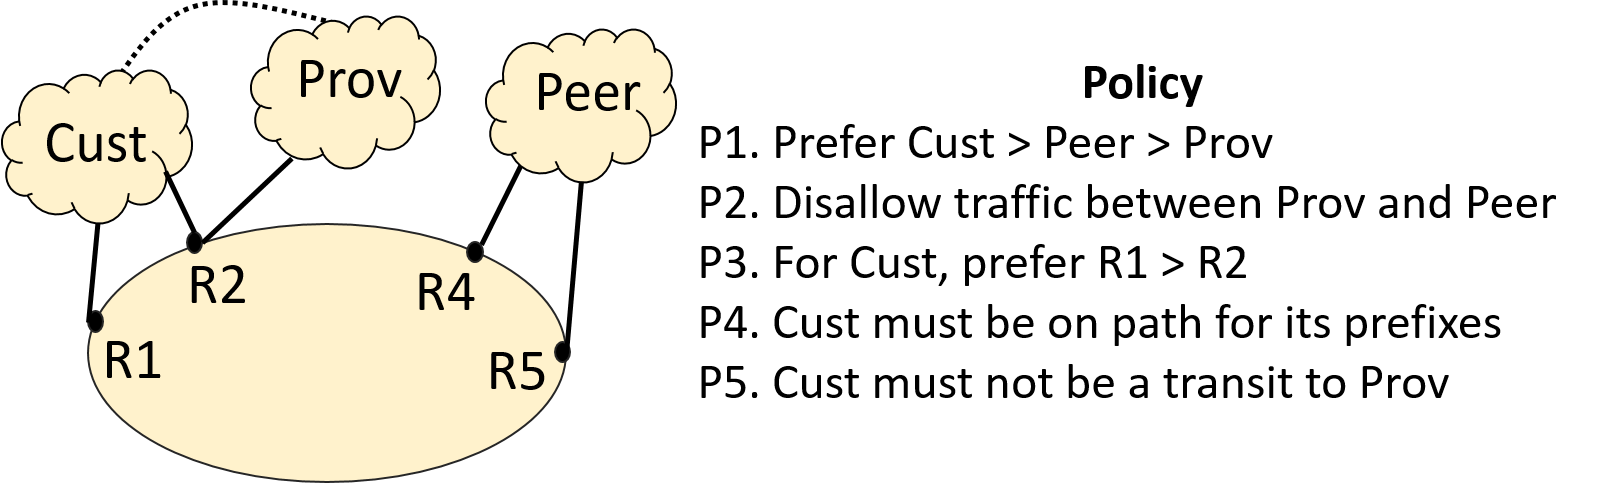
\includegraphics[width=\columnwidth]{figures/example1}
  \caption{Creating router-level policies is difficult.}
  \label{fig:example1}
  \vspace{-1em}
\end{figure}


\subsection{Example 1:  The backbone}

Consider the backbone network in Figure~\ref{fig:example1}. It has
three neighbors, a customer \CD{Cust}, a peer \CD{Peer}, and a provider \CD{Prov}. The policy of this network is shown on the right. It prefers that traffic leave the network through neighbors in a certain order (P1) and does not want to act as a transit between \CD{Peer} and \CD{Prov} (P2). It prefers to exchange traffic with \CD{Cust} over \CD{R1} rather than \CD{R2} because \CD{R1} is cheaper (P3). To guard against another AS "hijacking" prefixes owned by \CD{Cust}, the network only sends traffic to a neighbor if \CD{Cust} is on the AS path (P4). Finally, to guard against \CD{Cust} accidentally becoming a transit for \CD{Prov}, it does not use \CD{Cust} for traffic that will later traverse \CD{Prov} (P5).

To implement policy P1, the operators must compute and assign
local preferences such that preferences at \CD{Cust}-facing interfaces
$>$ \CD{Peer}-facing interfaces $>$ \CD{Prov}-facing interfaces. At
the same time, to satisfy P3, the preference at \CD{R2}'s
\CD{Cust}-facing interface should be lower than that at
\CD{R1}. Implementing P3 will also require MEDs to be appropriately configured on \CD{R1} and \CD{R2}.
To implement P2, the operators can assign communities that
indicate where a certain routing announcement entered the
network. Then, \CD{R4} must be configured to not announce to
$\CD{Peer}$ routes that have communities that correspond to the
\CD{R2}-\CD{Prov} link but to announce routes with communities for the \CD{R2}-\CD{Cust} and \CD{R1}-\CD{Cust} links. A similar policy must be configured for \CD{R2}. Finally, to implement P4 and P5, the operators will have to compute and configure appropriate prefix- and AS-path-based import and export filters at each router.

Clearly, it is difficult to correctly configure even this
small example network manually; correctly configuring real, larger networks can quickly become a nightmare. Such networks have hundreds of neighbors spanning multiple commercial-relationship classes, differing numbers of links to each neighbor, along with several neighbor- or prefix-based exceptions to the default behavior. A large AS with many peers in different geographic locations may be faced with complex challenges such as keeping traffic within national boundaries.
Templates help to an extent by keeping preference and community values consistent across routers, but operators must still do much of the conceptually difficult work manually.
%\sysname lets operators express such policies easily and intuitively. It then automatically generates per-device import and export filters, local preferences, MED attributes, and community tags to ensure that the policy is implemented correctly under all failure scenarios.

\begin{figure}[t!]
  \centering
  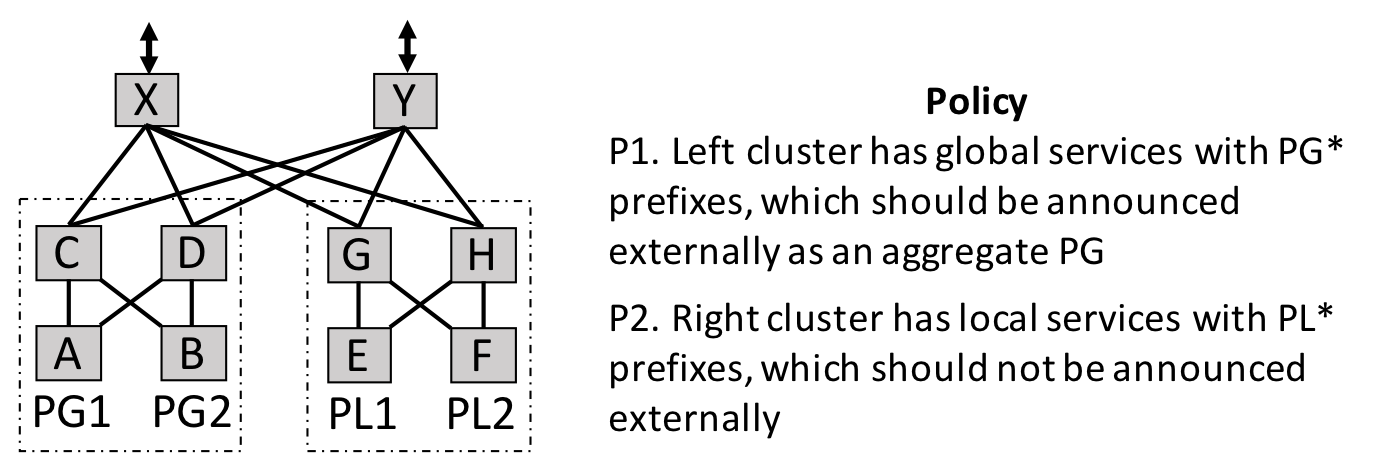
\includegraphics[width=\columnwidth]{figures/example2}
  \caption{Policy-compliance under failures is difficult.}
  \label{fig:example2}
  \vspace{-1em}
\end{figure}

\subsection{Example 2:  The datacenter}

 While configuring policies for a fully functional network is difficult, ensuring policy compliance in the face of failures can be almost impossible. Consider the datacenter network in Figure~\ref{fig:example2} with routers organized as a fat tree and running BGP.\footnote{For scale and policy flexibility, datacenter networks increasingly use BGP internally, with a private AS number per router~\cite{bgp-in-dc}.} The network has two clusters, one with services that should be reachable globally and one with services that should be accessible only internally. This policy is enabled by using non-overlapping address space in the two clusters and ensuring that only the address space for the global services is announced externally. Further, to reduce the number of prefixes that are announced externally, the global space is aggregated into a less-specific prefix \CD{PG}. The semantics of aggregation is that the aggregate prefix is announced as long as the router has a path to at least one sub-prefix.

The operator may implement the policy by having X and Y: $i)$ not export externally what they hear from G and H, routers that belong to the local services cluster; and $ii)$ export externally what they hear from routers C and D and aggregate to \CD{PG} if an announcement is subset of \CD{PG}. This implementation is appealing because X and Y do not need to be made aware of which prefixes are global versus local and IP address assignment can occur independently, e.g., local services can be assigned new prefixes without updating those routers' configurations.


However, this implementation has incorrect behavior in the face of failures. Suppose links X--G and X--H fail. Then, X will hear announcements for \CD{PL*} from C and D, having traversed from G and H to Y to C and D. Per its policy implementation, X will start "leaking" these prefixes externally. Depending on the rationale for local services, this leak could impact security (e.g., if the services are sensitive) or availability (e.g., if the \CD{PL*} prefixes are reused for other services outside of the datacenter). This problem does not manifest without failures because then X has and prefers paths to \CD{PL*} through G and H since they are shorter. A similar problem will happen if links Y--G and Y--H fail.
%\footnote{A different problem occurs when links X--C and X--D (or Y--C and Y--D) fail. X (Y) may stop announcing the global prefixes because they would be heard through G and H.}
Link failures in datacenters are frequent and it is not uncommon to have multiple failed links at a given time~\cite{dc-failure-study}.

To avoid this problem, the operator may disallow "valley" paths, i.e., those that go up, down, and back up again. This guard can be implemented by $X$ and $Y$ rejecting paths through the other. But that creates a different problem in the face of failures---an aggregation-induced blackhole~\cite{route-aggregation}. If links D--A and X--C fail, X will hear announcements for \CD{PG2} from D and will thus announce \CD{PG} externally. This announcement will bring to X traffic for \CD{PG1} as well, but because valleys are disallowed, X does not have a valid route for \CD{PG1} and will drop all traffic to it.

Thus, we see that devising a configuration that ensures policy compliance in the face of failures is complex and error-prone. \sysname lets operators implement their high-level policy specification in a way that guarantees compliance under all failures if possible---otherwise, it generates a compile-time error. For aggregation, it also provides a lower bound to operators on the number of failures under which aggregation will not result in blackholes.



%\subsection{OLD -- Overview}
%\todo{this subsection can be deleted once we have captured everything in it}
%
%Sources of bugs we fix. (It seems like the main advantage of our approach is not just fixing bugs though - it is easily describing high-level intention).
%Perhaps the best way to do this is by going through a bunch of examples in section 2 and showing how you could easily introduce bugs:
%
%\begin{itemize}
% \item Out of sync, or copy paste errors due to replicated configs (never an issue due to centralized control)
% \item Correct filtering to ensure no undesired traffic can flow through the network (e.g., best practices, like an AS should filter customers for their prefix, are implemented automatically )
% \item Failures can easily lead to unexpected behavior (e.g., a datacenter failure scenario w/instability.)
% \item Trying to do anything interesting, like get backups correct is difficult (e.g., setting up aggregation wrong)
% \item Related to the last point, things like aggregation can introduce black holes. We have the information needed to prevent this
%\end{itemize}
%
%
%Possible Examples:
%\begin{itemize}
% \item Basic datacenter with spine preference
% \item Simple AS that prefers customers over peers over providers
% \item Combined internal backup routing with preference based entrance into the network using aggregation.
% \item Something like cold potato routing
%\end{itemize}





%=====================================================
%
%
%  **Propane Language**
%
%
%=====================================================

\section{Propane overview}
\label{sec:propane}

Policies for (distributed) control planes differ from data-plane
policies in a few important ways. First, they must account for all failures at compile time; there is
no controller at runtime, so the routers must be configured in advance to handle failures in a compliant manner.
%
In \sysname, we enable such specifications through {\em path preferences}, with the semantics that a less-preferred path is taken only when a higher-preference path is unavailable in the network.
%
Second, paths in a control-plane policy may be under-specified (e.g.,
"prefer customer" does not indicate a concrete path). The \sysname
compiler treats such under-specifications as constraints on the set of
allowed paths and automatically computes valid sets based on the topology.
%

This section introduces the \sysname language using the
examples from the previous section.
%, introducing key aspects of
%the \sysname language along the way.
The next section describes the complete syntax of the
language as well as our strategy for compiling it to
BGP.

\subsection{Example 1: The backbone}

%\sysname simplifies network configuration by allowing users to
%specify end-to-end forwarding paths and associating them with
%appropriate prefixes.  The \sysname compiler handles the task of
%generating low-level BGP configurations consistent with the user's
%specifications.  It automatically synthesizes
%import-export filters, local preferences, MED attributes, and community tags
%to ensure policy compliance under all possible failure scenarios.

\sysname lets operators configure the network with the
abstraction that they have centralized control over routing.
Specifically, the operator simply provides a set of high-level constraints
that describe the
paths traffic should---or should not---take and their relative preferences.
\sysname specifications are written modularly via a series
of declarations.
%These definitions allow users to express the three
%major elements of any \sysname specification:  \emph{prefixes},
%\emph{paths} and \emph{policies}.
For example, to begin specification of the backbone
network from the previous section, we first express the idea that
we prefer that traffic leave the network through \CD{R1} over \CD{R2} (to \CD{Cust}) over \CD{Peer} over \CD{Prov} (policy P3 from Figure~\ref{fig:example1}):
%\begin{lstlisting}[mathescape=true]
%define ExitCust = $exit(R_1 \gg R_2)$
%\end{lstlisting}
\begin{code}
\Define Prefs = \Exit(R1 \Prefer R2 \Prefer Peer \Prefer Prov)
\end{code}
This  statement defines a set of \emph{ranked paths}, which includes
all paths (and only those paths) for which traffic exits our network
through either router \CD{R1}, router \CD{R2}, \CD{Peer}, or \CD{Prov}.
The paths that exit through \CD{R1}
are preferred (\Prefer) to those that exit through \CD{R2}, which are preferred to those that
leave through \CD{Peer} and then \CD{Prov}.  As we
describe in the next section, the \Exit\ predicate, as well as other
path predicates used later in this section, is simply a shorthand for
a particular regular expression over paths that is expressible in our policy
language. The preference operator (\Prefer) is flexible and can be used between constraints as well as among individual routers. For example, the above constraint could have been written equivalently as
\Exit(\CD{R1}) \Prefer \ldots \Prefer ~\Exit(\CD{Prov})

To associate ranked paths with
one or more prefixes, we define a \sysname \emph{policy}.
Within a policy, statements with the form $t\;$\Path$\;p$
associate the prefixes defined by the predicate $t$ with the set of
ranked paths defined by the path expression $p$.  In general,
prefix predicates can be defined by arbitrary boolean combinations
(and, or, not) of concrete prefixes and community tags.  Here,
we assume we have already defined the predicate \CD{PCust} for the
customer prefixes.
%and \CD{PInt} for our internal prefixes.
In the following code, ranked paths are associated with
customer prefixes,
and all other prefixes (\CD{true}). Policy statements are processed in
order with earlier policy statements taking precedence over later
policy statements. Hence, when the predicate \True{} follows
the statement involving \CD{PCust}, it is interpreted as
\CD{\True{} \AND{} \NOT{}PCust}.

%% \begin{lstlisting}[mathescape=true]
%% define Routing = {
%%     $\path{C_{pfx}}{ExitCust \gg end(Cust)}$
%%     $\path{I_{pfx}}{end(in)}$
%%     $\path{true}{ExitCust \gg exit(Peer) \gg exit(Prov)}$
%% }
%% \end{lstlisting}

\begin{code}
\Define Routing =
    \{PCust \Path Prefs \AND \End(Cust)
     \True  \Path Prefs \}
\end{code}
\noindent

Line 2 of this policy
restricts traffic destined to known customer prefixes (\CD{PCust}) to only follow paths that end at the customer. In addition, it enforces the network-wide preference that traffic leaves through \CD{R1} over \CD{R2} over \CD{Peer} over \CD{Prov}.
%defines the paths that exit our network to customer prefixes---\CD{ExitCust} defines paths through \CD{R1} and \CD{R2}, and in the event
%that connections to the customer through both routers fail,
%a backup route (\CD{\End(Cust)}) is defined that admits traffic along
%any path (including those through other networks) that ends at the customer.
%Line 3 states that traffic for internal prefixes must end in our network, and is otherwise unconstrained.
Line 3 applies to any other traffic not matching \CD{PCust} and allows the traffic to leave through any direct neighbor with the usual preferences of \CD{R1} over \CD{R2} over \CD{Peer} over \CD{Prov}. To summarize our progress, the \CD{Routing} policy
implements P1, P3, and P4 from Figure~\ref{fig:example1}.


Since, by default, routing allows transit traffic (\EG, traffic entering from
\CD{Peer} and leaving through \CD{Prov}), we separately define a
policy to enforce P2 and P5 from Figure~\ref{fig:example1}, using conjunction (\AND),
disjunction (\OR) and negation (\NOT) of constraints.
First, we create reusable abstractions for describing traffic that transits our network. In \sysname, this is done by creating a new parameterized definition.
\begin{code}
\Define transit(X,Y) = \Enter(X{\OR}Y) \AND \Exit(X{\OR}Y)
\Define cust-transit(X,Y) = \Later(X) \AND \Later(Y)
\end{code}
\noindent
Here we define transit traffic between groups of neighbors $X$ and $Y$ as traffic that enters the network through some neighbor in $X$ or $Y$ and then leaves the network through some neighbor in either $X$ or $Y$. Similarly, we define customer transit for customer $X$ and provider $Y$ as traffic that later goes through both $X$ and $Y$ after leaving our network. Using these two new abstractions, we can now implement policies P2 and P5 with the following constraint.

\begin{code}
\Define NoTrans =
  \{\True \Path \NOT{}transit(Peer,Prov) \AND
           \NOT{}cust-transit(Cust,Prov)\}
\end{code}
\noindent
The \CD{NoTrans} constraint requires that all traffic not follow a path that transits the network between \CD{Peer} and \CD{Prov}.
Additionally, it prevents traffic from ever following paths that leave our network and later go through both \CD{Prov} and \CD{Cust}.  To implement both \CD{Routing}
and \CD{NoTrans} simultaneously, we simply conjoin them: \CD{Routing \AND{} NoTrans}.
%
%% \begin{lstlisting}[mathescape=true]
%% Routing $\AND$  NoTransit
%% \end{lstlisting}
%

Collectively, the constraints above capture the entire policy. From them, our compiler will generate per-device import and export filters, local preferences,
MED attributes, and community tags to ensure that the policy is
implemented correctly under all failures.

\subsection{Example 2: The datacenter}

Our datacenter example network has three main concerns:
(1) traffic for the prefix allocated to each top-of-rack router must be able to reach that router,
(2) local services must not leak outside the datacenter, and
(3) aggregation must be performed on global prefixes to reduce churn
in the network.

\sysname allows modular specification of each of these constraints. The first constraint is about prefix ownership---we want traffic only for certain prefixes to end up at a particular location. The following definition captures this intent.

%% \begin{lstlisting}[mathescape=true]
%% define Ownership = {
%%     $\path{p_{g1}}{end(A)}$
%%     $\path{p_{g2}}{end(B)}$
%%     $\path{p_{l1}}{end(E)}$
%%     $\path{p_{l2}}{end(F)}$
%% }
%% \end{lstlisting}

\begin{code}
\Define Ownership =
    \{PG1 \Path \End(A)
     PG2 \Path \End(B)
     PL1 \Path \End(E)
     PL2 \Path \End(F)
     \True \Path \End(\Out)\}
\end{code}
\noindent
This definition says that traffic for prefix \CD{PG1} is allowed to follow only paths that
end at router \CD{A}; traffic for \CD{PG2},
but not \CD{PG1}, must
end at router \CD{B}; and so on.
Any traffic destined for a prefix that not a part of the datacenter should be allowed to leave the datacenter and end at some external location, which is otherwise unconstrained.
The special keyword \Out{} matches any location outside the datacenter network, while the keyword \In{} will match any location inside the network.

For the second constraint, we define another policy:

%% \begin{lstlisting}[mathescape=true]
%% define Routing = {
%%     $\path{p_{g*}}{any}$
%%     $\path{p_{l*}}{\NOT enter(out)}$
%%     $\path{true}{exit(out)}$
%% }
%% \end{lstlisting}
\begin{code}
\Define Locality =
    \{PL1 \OR PL2 \Path \textbf{only}(\In)\}
\end{code}
\noindent
%The first line states that there is no restriction (\Any)
%on how traffic must traverse the network for global prefixes.
%aside from the default restriction
%that traffic must not pass through the user's network and then loop
%back on itself.
%This means traffic for
%\CD{PG*} may be sent either from other datacenter routers or
%from external ASes.
This definition says that traffic for local
prefixes only follows paths that are internal to the network at each hop.
This constraint guarantees that the services remain reachable only to locations
inside the datacenter.

As in the backbone example, we can logically conjoin these constraints
to specify the network-wide policy.
However, in addition to constraints on the shape of paths,
\sysname allows the operator to specify constraints on the BGP control plane itself.
For instance, a constraint on aggregation is included to ensure that
aggregation for global prefixes is performed from
locations inside (\In) the network to locations outside (\Out).
In this case, \CD{PG1} and \CD{PG2} will use the aggregate \CD{PG}
(which we assume is defined earlier)
when advertised outside the datacenter.

\begin{code}
Ownership \AND{} Locality \AND{} \Agg(PG, \In \Link \Out)
\end{code}

Once \sysname compiles the policy, it is guaranteed to remain compliant under all possible failure scenarios, modulo any aggregation-induced black holes. In the presence of aggregation, the \sysname compiler will also efficiently find a lower bound on the number of failures required to create an aggregation-induced black hole.


%%%%OLD TEXT BELOW
%
%\section{Propane}
%\label{sec:propane}
%
%\sysname simplifies network configuration by automatically generating low-level BGP configurations from a high-level specification of the network's routing policy.
%%
%The operator configures the network with the abstraction that he or she has centralized control over routing and uses a set of high-level constraints to describe the different routes traffic may (or may not) take and their relative preferences.
%%
%The \sysname compiler generates BGP configurations for each device in the network that operate in a completely distributed fashion and are correct by construction -- automatically synthesizing import/export filters, local preference and MED attributes, and community tags to ensure policy compliance under all possible failure scenarios.
%%
%We now demonstrate \sysname by showing how to configure the networks from the previous examples.
%
%\para{Example 1}
%
%We now show how to write the routing policy for the backbone network in Section~\ref{sec:motivation}. \sysname allows to address each of the requirements in turn. First we address requirements (P1), (P3), and (P4) that customers are preferred over peers over providers, and that a customer appear on the path for its prefix. The following \sysname code accomplishes these two objectives:
%
%\begin{lstlisting}[mathescape=true]
%define ExitCust = $exit(R_1 \gg R_2)$
%
%define Routing = {
%    $\path{C_{pfx}}{ExitCust \gg end(Cust) }$
%    $\path{I_{pfx}}{end(in)}$
%    $\path{true}{ExitCust \gg exit(Peer) \gg exit(Prov)}$
%}
%\end{lstlisting}
%
%The first definition defines paths that exit our network to the customer. The statement $exit(R_1 \gg R_2)$ restricts us to paths that leave our network through either router $R_1$ or $R_2$, with a preference for $R_1$.
%The first line of the \textsf{Routing} policy ensures that traffic destined for customer prefixes ($C_{pfx}$) either leaves the network directly to the customer (with a preference for leaving through $R_1$), or simply ends at the customer. Not leaving directly to the customer by going through \textit{Peer} or \textit{Prov} is less preferred than leaving directly, and thus serves as a backup route in a direct route is not available.
%
%The second line state that traffic for internal prefixes $I_{pfx}$ must end in our network, and is otherwise unconstrained. The last line applies to any other traffic, and allows for any routes that leave through a peer with a preference for customers over peers over providers. While this still allows transit traffic (e.g., traffic can enter from \textit{Peer} and leave through \textit{Prov}), we can restrict this behavior separately as follows:
%
%\begin{lstlisting}[mathescape=true]
%define PP = Peer or Prov
%define PPTransit = $enter(PP) \wedge exit(PP)$
%define CustTransit = $later(Cust) \wedge later(Prov)$
%
%define NoTransit = {
%    $\path{true}{\neg PPTransit \wedge \neg CustTransit}$
%}
%\end{lstlisting}
%
%The \textsf{NoTransit} constraint above ensures that requirements (P2) and (P5) are satisfied. In particular, it says that, for any prefix, traffice should never both enter and exit the network from \textit{Peer} or \textit{Prov}. Similarly it prevents traffic from ever following paths that leave our network and later go through both \textit{Prov} and \textit{Cust}.
%
%\begin{lstlisting}[mathescape=true]
%Routing $\wedge$  NoTransit
%\end{lstlisting}
%
%The final policy is simply the conjunction of the routing and no transit constraints. \sysname will generate per-device import and export filters, local preferences and MED attributes, and community tags to ensure that the policy is met under all failure scenarios.
%
%
%\para{Example 2}
%
%Consider again the datacenter from Section~\ref{sec:motivation}. In this example, there are primarily three main concerns: (1) traffic for the prefix block allocated to each top-of-rack router can reach that router, (2) local services do not leak outside the datacenter, and (3) aggregation is performed on global prefixes to reduce churn in the network.
%
%\sysname allows us to decompose and specify each of these constraints in a modular fashion. The first constraint is about prefix ownership -- namely, that we only want traffic for certain prefixes to end up at a particular locations. The following definition in propane captures this intent:
%
%\begin{lstlisting}[mathescape=true]
%define Ownership = {
%    $\path{p_{g1}}{end(A)}$
%    $\path{p_{g2}}{end(B)}$
%    $\path{p_{l1}}{end(E)}$
%    $\path{p_{l2}}{end(F)}$
%}
%\end{lstlisting}
%
%The constraints in the ownership task are read in a top-down fashion. Traffic for prefix $p_{g1}$ is only allowed to to follow paths that end at router A. Similarly, traffic not matching $p_{g1}$, but which matches $p_{g2}$ must end at router B and so on.
%%
%To capture the second constraint, we can define another task for the core routing policy:
%
%\begin{lstlisting}[mathescape=true]
%define Routing = {
%    $\path{p_{g*}}{any}$
%    $\path{p_{l*}}{\neg enter(out)}$
%    $\path{true}{exit(out)}$
%}
%\end{lstlisting}
%
%The first line states that there is no restriction on how traffic must traverse the network for global prefixes. This means traffic for $p_{g*}$ may be sent either from other routers in the datacenter, or from external ASes. The second line ensures that traffic for local prefixes never enters the network from an outside location. This  guarantees that the services remain reachable only to locations internal to the datacenter.
%
%Finally, we can combine these constraints logically to specify the network-wide policy:
%
%\begin{lstlisting}[mathescape=true]
%Ownership $\wedge$ Routing $\wedge$ agg($p_{agg}$, $in \rightarrow out$)
%\end{lstlisting}
%
%
%In addition to constraints on the shape of paths, \sysname allows the operator to specify constraints on the BGP control plane. Above, a constraint on aggregation is included to ensure that an aggregation for $p_{agg}$ is performed from locations inside the network to locations outside the network.
%
%Once \sysname compiles the policy, it is guaranteed to hold under all possible failure scenarios. Similarly, it can check for aggregate-induced black holes up to $k$ failures.
%




%=====================================================
%
%
%  **Compilation**
%
%
%=====================================================

\section{Compilation}
\label{sec:compilation}

The examples above use what we call the front end (FE) of \sysname.
It simplifies operators' task of describing preferred paths, but that simplicity comes at the cost of compilation complexity. The compiler must efficiently compute the sets of paths represented by the intersection of preferences and topology, determine which ones can be honored under failures, and ensure policy compliance under all failure cases.

\begin{figure}[t!]
  \centering
  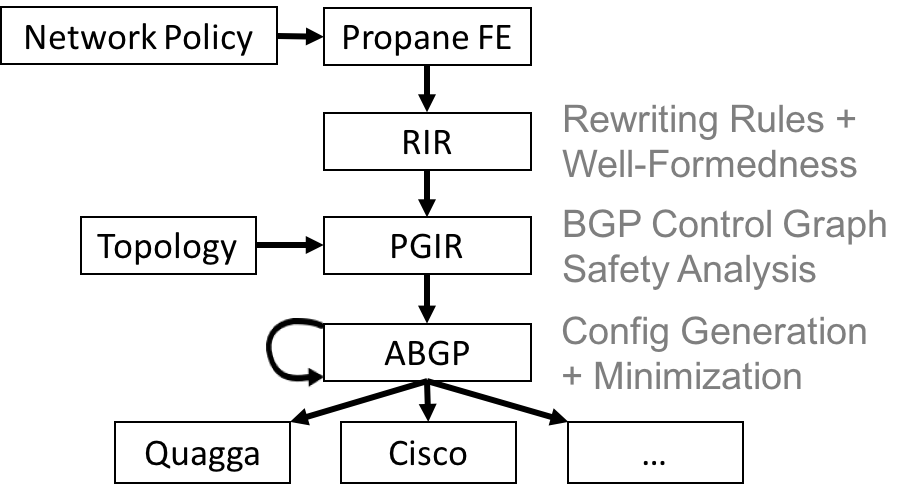
\includegraphics[width=.75\columnwidth]{figures/pipeline}
  \caption{Compilation pipeline stages for Propane.}
  \label{fig:pipeline}
  \vspace{-1em}
\end{figure}

% grammar
\newcommand{\BNFALT}{\;\;|\;\;}
\newcommand{\hdr}[2]{\flushleft \chdr{\hspace{5mm}#1}{#2}}
\newcommand{\chdr}[2]{\textbf{#1} {#2} \\ \centering}

\begin{figure*}[t]\small
  \begin{minipage}[t]{.45\linewidth}
  \hdr{Syntax}{}
  \vspace*{-1\baselineskip}
  %
  \[ \begin{array}{rclr}
    \hline

     pol     &::=& p_1, \dots, p_n & \textit{constraints} \\
     p       &::=& t \hspace{.3em} \Path \hspace{.3em} r_1 \Prefer \dots \Prefer r_m & \textit{preferences} \\
     x       &::=& d.d.d.d/d & \textit{prefix} \\
     t       &::=& \True & \textit{true} \\
         &\BNFALT& \NOT t & \textit{negation} \\
         &\BNFALT& t_1 \OR{} t_2 & \textit{disjunction} \\
         &\BNFALT& t_1 \AND{} t_2 & \textit{conjunction} \\
         &\BNFALT& \textit{prefix} = x & \textit{prefix test} \\
         &\BNFALT& \textit{comm} = d & \textit{community test} \\
     r       &::=& n & \textit{AS number} \\
         &\BNFALT& \emptyset & \textit{empty set} \\
         &\BNFALT& \In & \textit{internal loc} \\
         &\BNFALT& \Out & \textit{external loc} \\
         &\BNFALT& r_1 \cup r_2 & \textit{union} \\
         &\BNFALT& r_1 \cap r_2 & \textit{intersection} \\
         &\BNFALT& r_1 \cdot r_2 & \textit{concatenation} \\
         &\BNFALT& \NOT r & \textit{path negation} \\
         &\BNFALT& r^* & \textit{iteration} \\
     l       &::=& r_1 \rightarrow r_2 & \textit{link pairs} \\
     cc     &::=& agg(x, l) \BNFALT tag(c, t, l) & \textit{control constraints} \\
  \end{array} \]

  \end{minipage}
  %
  ~~
  \vrule
  ~~
  %
  \begin{minipage}[t]{.5\linewidth}\small
  \hdr{Propane Expansions}{}
  \vspace*{-1\baselineskip}
  %
  \[\begin{array}{rcl}
    \hline
    \Any           & = & \Out^* \cdot \In^+ \cdot \Out^* \\
    \None          & = & \emptyset \\
    \Internal      & = & \In^+ \\
    \Only(X)       & = & \Any \cap X^* \\
    \Never(X)      & = & \Any \cap (!X)^* \\
    \Through(X)    & = & \Out^* \cdot \In^* \cdot X \cdot \In^* \cdot \Out^* \\
    \Later(X)      & = & \Out^* \cdot (X \cap \Out) \cdot \Out^* \cdot \In^+ \cdot \Out^* \\
    \Before(X)     & = & \Out^* \cdot \In^+ \cdot \Out^* \cdot (X \cap \Out) \cdot \Out^* \\
    \End(X)        & = & \Any \cap (\Sigma^* \cdot X) \\
    \Start(X)      & = & \Any \cap (X \cdot \Sigma^*) \\
    \Exit(X)       & = & (\Out^* \cdot \In^* \cdot (X \cap \In) \cdot \Out \cdot \Out^*) \cup \\
                  &        & (\Out^* \cdot \In^+ \cdot (X \cap \Out) \cdot \Out^*) \\
    \Enter(X)      & = & (\Out^* \cdot \Out \cdot (X \cap \In) \cdot \In^* \cdot \Out^*) \cup \\
                  &        & (\Out^* \cdot (X \cap \Out) \cdot \In^+ \cdot \Out^*) \\
    \LinkKW(X,Y)     & = & \Any \cap (\Sigma^* \cdot X \cdot Y \cdot \Sigma^*) \\
    \PathKW(\vec{X}) & = & \Any \cap (\Sigma^* \cdot X_1 \dots X_n \cdot \Sigma^*) \\
    \Novalley(\vec{X}) & = & \Any ~ \cap \\
                  &   & \NOT\PathKW(X_2,X_1,X_2) ~ \cap \dots \cap \\
                  &   & \NOT\PathKW(X_n,X_{n-1},X_n) \\
  \end{array} \]

  \end{minipage}

  \hrulefill

  \caption{Regular Intermediate Representation (RIR) syntax (left), and
           Propane language expansions (right).}
  \label{fig:rir-syntax}
  %\vspace{-1em}
\end{figure*}

To handle these challenges, we decompose compilation into multiple stages, shown in  Figure~\ref{fig:pipeline}, and develop efficient algorithms for the translation between stages. The first stage of the pipeline involves simple rewriting rules and substitutions from the FE to the core Regular Intermediate Representation (RIR). Policies in RIR are checked for well-formedness (\EG, never constraining traffic that does not enter the network), before being combined with the network topology to obtain the Product Graph Intermediate Representation (PGIR). The PGIR is a data representation that compactly captures the flow of BGP announcements subject to the policy and topology restrictions. We develop efficient algorithms that operate over the PGIR to ensure policy compliance under failures, avoid BGP instability, and prevent aggregation-induced black holes. Once the compiler determines safety, it translates the PGIR to an abstract BGP (ABGP) representation. ABGP can then be translated into various vendor-specific device
configurations as needed.
%The \sysname compiler currently generates
% Quagga router configurations from ABGP.

\subsection{Regular IR (RIR)}
\label{sec:rir}

%\para{Syntax}
The \sysname FE is just a thin layer atop the RIR for describing preference-based path constraints.
Figure~\ref{fig:rir-syntax} shows the RIR syntax. A policy has one or more constraints, each of which has a test on the type of route, and a corresponding set of preferred regular paths. Regular paths are regular expressions where the base characters are abstract locations---either a router or an AS. Special \In{} and \Out{} symbols refer to any internal or external location respectively. In addition, $\Sigma$ refers to any symbol. We also use the standard regular expressions abbreviation $r^+$ for $r \cdot r^*$, a sequence of one or more occurrences of $r$. Predicates ($t$) consist of logical boolean connectives (and, or, not) as well as tests that match a particular prefix (or group of prefixes) and tests for route advertisments with a particular community value (i.e., an integer value associated with a path).
%% For example, the constraint
%% \[(\textit{prefix}=74.3.28.0/24) \Link \\
%% (as200 \cdot \In^+) \Prefer (as100 \cdot \In^+)
%% \]
%% describes a more-preferred set of paths for traffic announced by a prefix no less specific than \CD{74.125.28.0/24}, which starts at AS 200, before entering and staying inside the user's network to get to the destination, and a less-preferred set of paths that start at AS 100 and are otherwise the same. The plus operator $\In^+$ stands for $\In \cdot \In^*$, at least one internal hop. Tests over route types use standard boolean connectives, and can refer to both prefixes and route community values.

\sysname also supports constraints purely on the control-plane behavior of BGP. For example, prefix aggregation is an important optimization to reduce routing table size and churn in practice. A constraint of the form $agg(x,l)$ tells the compiler to perform aggregation for prefix $x$ across all links described by $l$. It is also often useful to be able to add community tags to exported routes in BGP (e.g., to communicate non-standard information to peers). A constraint of the form $tag(c,t,l)$ adds community tag $c$ for any prefixes matching $t$ across links $l$.
%% Aggregation, for example, from internal to external locations, is specified using the same regular syntax as before:
%% $$\Agg(128.17.0.0/16, \In \Link \Out)$$
%% where the expression $\In \Link Out$ refers to control messages flowing from any internal to any external location.
We list only the route aggregation and community tagging constraints in Figure~\ref{fig:rir-syntax}, but we also support other constraints such as limiting the maximum number of routes allowed between ASes, or enabling BGP multipath.


\para{Semantics}

The semantics of RIR is in terms of ranked paths. Each preference-based regular path constraint of the form $r_1 \Prefer \dots \Prefer r_j$ maps to a set of concrete paths in the network that match one of $r_i$. A network path is a string of abstract locations of the form $n_1 n_2 \dots n_k$. A regular expression $r$ matches path $p$, if $p \in \mathcal{L}(r)$, that is, the path is in the language of the regular expression and is topologically valid.
%We denote the length of a path $p$ as $\abs{p}$.

A path $p$ has rank:
$$(\min_i \set{ p \in \mathcal{L}(r_i) }, \abs{p})$$
which is lexicographically ordered according to (1) the most preferred regular expression matched, and (2) as a tie breaker, the path length $\abs{p}$. Lower ranks indicate \emph{more} preferred paths. Traffic may be sent on any of the most preferred paths for each pair of starting and ending locations that appear in some specified path. There is an implicit lowest preference $\emptyset$ to drop traffic when no other route is possible.

The set of ranked paths depends on which paths are valid in the topology, and thus when failures occur, the most preferred routes change. The \sysname compiler ensures that generated configurations for a policy always achieve the most preferred path possible given the failures in the topology, using only distributed mechanisms.


\para{From FE to RIR}

The first stage in \sysname compilation reduces the FE to the simpler RIR from Figure~\ref{fig:rir-syntax}.
The main differences between the FE and RIR are: $i)$ FE allows the programmer to specify constraints using a series of (modular) definitions, and combine them later, $ii)$ FE provides high-level names that abstract sets of routes and groups of prefixes/neighbors, and $iii)$ FE allows the preference operator to be used more flexibly.

A key constraint when translating FE to RIR is ensuring that all specified routes are well-formed. In particular, each regular path constraint $r$ must satisfy $r \subseteq \Out^* \cdot \In^+ \cdot \Out^*$. It ensures that users only control traffic that goes through their network at some point, and that such traffic does not loop back multiple times through their network.

The translation from FE to RIR is based on a set of rewriting rules.
The first step merges separate constraints. It takes the cross product of per-prefix constraints, where logical conjunction ($a \AND b$) is replaced by intersection on regular constraints ($a \Intersect b$), logical disjunction is replaced by union, and logical negation ($\NOT a$) is replaced by path negation ($\Any \cap \NOT(a)$). The additional constraint $\Any$ ensures the routes are well-formed by restricting the paths to only those that go through the user's network.
%
For example, in the datacenter configuration from \S\ref{sec:propane}, combining the \CD{Locality} and \CD{Ownership} policies results in the following RIR:

%% \begin{lstlisting}[mathescape=true]
%% $\path{p_{g1}}{any \cap end(A)}$
%% $\path{p_{g2}}{any \cap end(B)}$
%% $\path{p_{l1}}{\neg enter(out) \cap end(E)}$
%% $\path{p_{l2}}{\neg enter(out) \cap end(F)}$
%% $\path{true}{exit(out)}$
%% \end{lstlisting}

\begin{code}
PG1 \Path \End(A)
PG2 \Path \End(B)
PL1 \Path \textbf{only}(\In) \Intersect \End(E)
PL2 \Path \textbf{only}(\In) \Intersect \End(F)
\True \Path \Exit(\Out)
\end{code}

The next step rewrites the high-level constraints such as $\Enter$ according to the equivalences in Figure~\ref{fig:rir-syntax}. Since preferences can only occur at the outermost level for an RIR expression, the final step is to ``lift" occurrences of the preference operator in each regular expression. For example, the regular expression $a \cdot (b \Prefer c) \cdot d$ is lifted to $(a \cdot b \cdot d) \Prefer (a \cdot c \cdot d)$ by distributing the preference over the sequence operator. In general, we employ the follwing distributivity equivalences:
%
\[
\begin{array}{c}
  x \odot (y_1 \Prefer \dots \Prefer y_n) = (x \odot y_1) \Prefer \dots \Prefer (x \odot y_n) \\
  (y_1 \Prefer \dots \Prefer y_n) \odot x = (y_1 \odot x) \Prefer \dots \Prefer (y_n \odot x)
\end{array}
\]
%
where $\odot$ stands for an arbitrary regular binary operator, and $x$ is a policy with a single preference. The compiler flags as invalid preferences nested under a unary operator (i.e., \textit{star} or \textit{negation}).





\newcommand{\state}[4]{\node[state,#3](#1)[#4]{#2};}
\newcommand{\transition}[4]{\path[->] (#1) edge [#4] node {#3} (#2);}

\begin{figure*}
  \begin{minipage}[t]{.5\linewidth}

  \hdr{Topology}{}
  \vspace*{-2\baselineskip}

  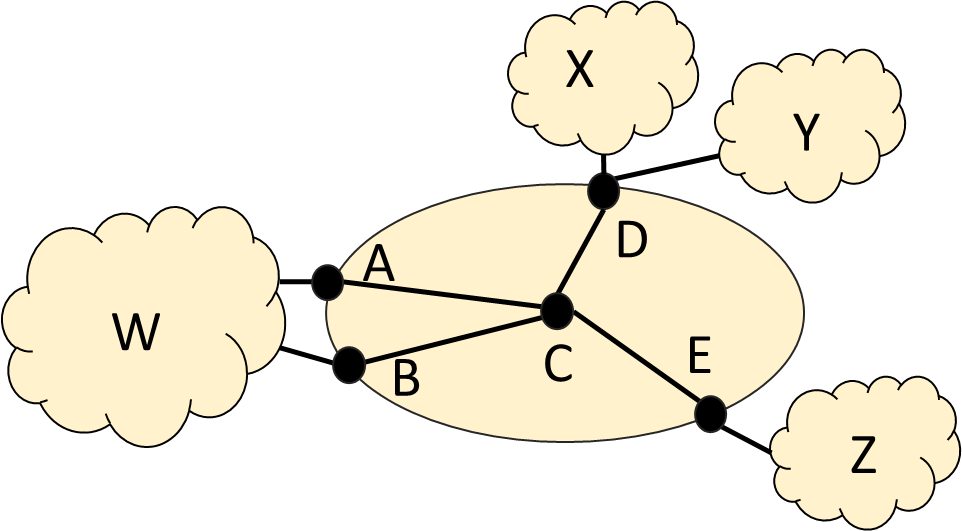
\includegraphics[width=.6\columnwidth]{figures/topology}

  \hdr{Policy Automata}{}
  \vspace*{-0.5\baselineskip}

  \begin{tikzpicture}[>=stealth',shorten >=1pt,auto,node distance=1.4cm,minimum size=1cm]
    \state{0}{$0$}{              }{}
    \state{1}{$1$}{right of=0}{}
    \state{2}{$2$}{right of=1}{}
    \state{3}{$3$}{right of=2}{}
    \state{4}{$4$}{right of=3}{}
    \state{5}{$5$}{right of=4}{accepting}
    \transition{0}{1}{out}{}
    \transition{1}{2}{D}{}
    \transition{2}{3}{C}{}
    \transition{3}{4}{A}{}
    \transition{4}{5}{W}{}
  \end{tikzpicture}

  \begin{tikzpicture}[>=stealth',shorten >=1pt,auto,node distance=1.6cm]
    \state{0}{$0$}{              }{}
    \state{1}{$1$}{right of=0}{}
    \state{2}{$2$}{right of=1}{}
    \state{3}{$3$}{right of=2}{}
    \state{4}{$4$}{right of=3}{accepting}
    \transition{0}{1}{out}{}
    \transition{1}{2}{in}{}
    \transition{2}{2}{A,C,D,E}{loop above}
    \transition{2}{3}{B}{}
    \transition{3}{3}{B}{loop above}
    \transition{3}{2}{A,C,D,E}{bend left}
    \transition{3}{4}{W}{}
  \end{tikzpicture}
  \end{minipage}
  %
  ~~
  ~~
  %
  \begin{minipage}[t]{.5\linewidth}
  \hdr{Product Graph IR}{}
  \vspace*{-1\baselineskip}
  %
  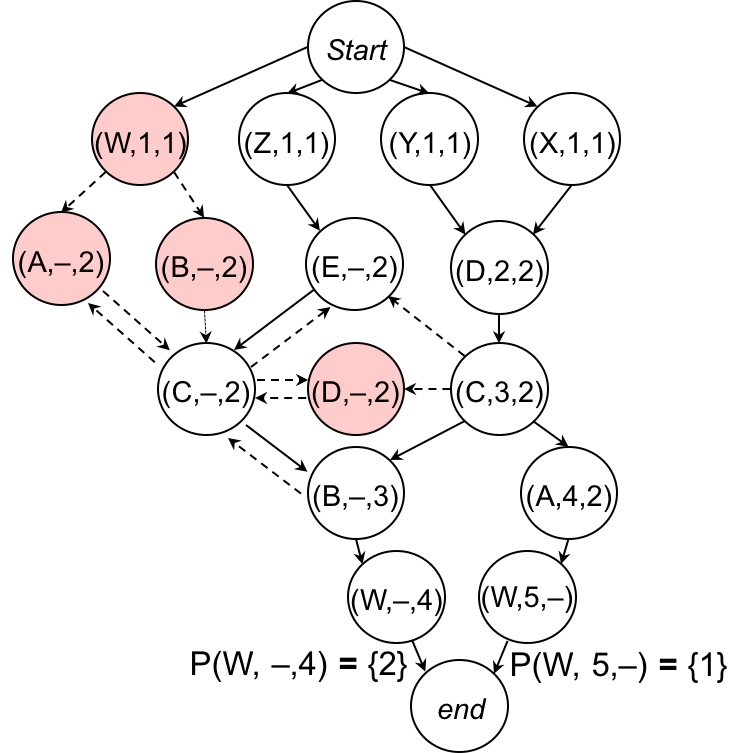
\includegraphics[width=.65\columnwidth]{figures/productgraph}
  \end{minipage}

  \hrulefill
  \vspace*{.4em}

  \caption{Example Product Graph IR construction for policy: $(\CD{W} \cdot \CD{A} \cdot \CD{C} \cdot \CD{D} \cdot \Out) \Prefer (\CD{W} \cdot \CD{B} \cdot \In^+ \cdot \Out)$.}
  \label{fig:example-compilation}
  %\vspace{-1em}
\end{figure*}


\subsection{Product graph IR}

Now that the user policy exists in a simplified form, we must consider the topology. In particular, we want a compact representation that describes all the possible ways BGP route announcements can flow through the network subject to the policy and topology constraints. The PGIR captures these constraints by ``intersecting" each of the regular automata corresponding to the RIR path preferences and the topology. Paths through the PGIR correspond to real paths through the topology that satisfy the user constraints.

%Finding paths through a graph subject to regular constraints has been studied extensively in the database literature~\ref{bib:todo}, and has been applied to networks in the past~\ref{bib:todo}.

\para{Formal definition}

% Formally define automata
%The RIR policy is an ordered sequence of regular expressions $r_1 \Prefer \dots \Prefer r_j$.
While paths in RIR policy describe the direction traffic flow through the network, to implement the policy with BGP we are concerned about the way control-plane information is disseminated, i.e., route announcements flowing in the opposite direction. To capture this idea, for each regular expression $r_i$ in RIR policy, we construct a deterministic finite state machine on the reversed regular expression. Each automaton for the reversed regular expression of $r_i$ is a tuple ($\Sigma, Q_i, F_i, q_{0_i}, \sigma_i$). The alphabet $\Sigma$ consists of all abstraction locations (i.e., routers or ASes), $Q_i$ is the set of states for automaton i, $F_i$ is the set of final states, $q_{0_i}$ is the initial state, and $\sigma_i \colon Q_i \times \Sigma \rightarrow Q_i$ is the state transition function.
%
% Formally define topology
The topology is represented as a graph ($V, E$), which consists of a set of vertices $V$, and a set of directed edges $E \colon V \times V$.
%
% Formally define product graph
The combined PGIR is a tuple ($V'$, $E'$, $s$, $e$, $P$) with
vertices $V' \colon V \times Q_1 \times \dots \times Q_j$,
edges $E' \colon V' \times V'$,
a unique starting vertex $s$,
a unique ending vertex $e$,
and a preference function $P \colon V' \rightarrow 2^{\set{1, \dots, j}}$ , which maps nodes in the product graph to a set of preference ranks.
For a PGIR vertex $v' = (v, \dots) \in V'$, we say $loc(v') = v$, which indicates that the corresponding topology location for $v'$ is $v$.
Two nodes $x$ and $y$ \emph{shadow} each other in the product graph when $x \in V'$ and $y \in V'$ and $loc(x) = loc(y)$.

\para{From RIR To PGIR}

% Formal product construction
Let $a_i$ and $b_i$ denote states in the regular policy automata.
The PGIR is constructed by adding an edge from $v_1 = (x, a_1, \dots, a_m)$ to $v_2 = (y, b_1, \dots, b_m)$ whenever $\sigma_i(a_i, y) = b_i$ for each $i$ and $(x,y) \in E$ is a valid topology link.
%
Additionally, we add edges from the start node $s$ to any $v = (x, a_1, \dots, a_m)$ when $\sigma_i(q_{0_i}, x) = a_i$ for each $i$.
%
The preference function $P$ for node $v = (x, a_1, \dots, a_m)$ is defined as $P(v) = \set{i~\vert~a_i \in F_i} $. That is, it records which preferences are achieved from each policy automaton for every node in the product construction.
%
Finally, there is an edge from each node in the PGIR such that $P(v) \neq \emptyset$ to the special end node $e$. We write $(x \leq_{rank} y)$ if either $P(x) = P(y) = \emptyset$ or $min ~ P(x) \leq min ~ P(y)$, which means that paths ending at PGIR node $x$ are better than (lower rank) than paths that ending at $y$.


Intuitively, PGIR tracks which states of each automaton the policy is in as route announcements move between locations.
%
Consider the topology in Figure~\ref{fig:example-compilation}. Suppose we want a primary route from neighbor W that allows traffic to enter the network at $A$, and utilize the C--D link before leaving the network (through $X$ or $Y$). As a backup, we also want to allow traffic to enter the network from $B$, in which case the traffic can also utilize the C--E link before leaving the network. For simplicity, we assume that the route ends in either $X$, $Y$, or $Z$. The RIR for the policy could be written as:
%
$$(\CD{W} \cdot \CD{A} \cdot \CD{C} \cdot \CD{D} \cdot \Out) \Prefer (\CD{W} \cdot \CD{B} \cdot \In^+ \cdot \Out)$$
%
Figure~\ref{fig:example-compilation} shows the policy automata for each regular expression preference. Since we are interested in the flow of control messages, the automata match backwards.
%
The figure also shows the PGIR after intersecting the topology and policy automata. Every path in the PGIR corresponds to a concrete path in the topology. In particular, every path through the PGIR that ends at a node $v$ such that the preference function $P(v) = \set{i_1, \dots, i_m}$ is non-empty, is a valid topological path that satisfies the policy constraints and results in a particular path with preferences $i_1$ through $i_m$.
%
For example, the path $X \cdot D \cdot C \cdot A \cdot W$ is a valid path in the topology that BGP route announcements might take, which would lead to obtaining a path with the lowest (best) rank of $1$.
BGP control messages can start from peer X, which would match the $\Out$ transition from both automata, leading to state $1$ in the first automaton, and state $1$ in the second automaton. This possiblity is reflected in the product graph by the node with state $(X,1,1)$. From here, if X were to advertise this route to D, it would result in the path $D \cdot X$, which would lead to state $2$ in the first automaton, and state $2$ in the second automaton, and so on.
%
The ``--" state indicates the corresponding automaton can not accept the current path or any extension of it. Since node $(W,5,-)$ is in an accepting state for the first automata, it indicates that this path has preference 1.

\para{Minimization}
After building the PGIR as desribed above,
we minimize it in order to improve the subsequent analysis that checks if the policies captured by it are safe under failures.
The minimization is based on the observation that, although every path in the PGIR is a valid path in the topology, we do not want to consider paths that form loops. In particular, BGP's loop prevention mechanism forces an AS to reject any route for which it is already in the AS path.
%
For example, in Figure~\ref{fig:example-compilation}, the path $W \cdot A \cdot C \cdot B \cdot W$ is a valid topological path, leading to a path that satisfies the preference 1 policy, but which contains a loop.
%
The precision of the failure-safety analysis often increases when nodes and edges that are not possible due to loops are eliminated.
%For example, if we can safely remove a PGIR edge, then we do not have to consider what happens when the edge has failed.

We use graph dominators~\cite{tarjan-dominance} as a cheap approximation for removing many nodes and edges in the PGIR that are never on any \emph{simple} (loop free) path between the start and end nodes.
In the PGIR, a node $x$ dominates a node $y$ if $x$ appears on every path leading from the start node to $y$. Similarly, a node $x$ post-dominates a node $y$ in the PGIR if $x$ appears on every path from $y$ to the end node.
We can safely remove nodes and edges in the PGIR when any of the following conditions hold, where $x$, $x'$ and $y$, $y'$ refer to PGIR nodes that shadow each other:
\begin{itemize}
\setlength{\itemsep}{1pt}
\setlength{\parskip}{0pt}
\setlength{\parsep}{0pt}
\item Remove $x$ if it is not reachable from the start node
\item Remove $x$ if it can not reach the end node
\item Remove $x$ if it is (post-)dominated by some $x'$
\item Remove edge ($x$, $y$) if $y$ is post-dominated by some $x'$
\item Remove edge ($x$, $y$) if $x$ is dominated by some $y'$
\end{itemize}
%We can safely remove any PGIR node or edge as long as it never appears on any \emph{simple} path from the \textit{start} node to the \emph{end} node.
For example, node $(W,1,1)$ in Figure~\ref{fig:example-compilation} can be removed since it is never on a simple path to the end node because it must always go through node $(W,-,4)$. That is, node $(W,-,4)$ post-dominates node $(W,1,1)$. We repeatedly apply the minimizations above to the PGIR until no further minimization is possible.
In the example of Figure~\ref{fig:example-compilation}, colored nodes and dashed edges are removed after minimization.
 %since they are irrelvant to the BGP decision process.
%
%Although fully minimizing this graph is an NP-complete problem,  a simple and efficient algorithm based on graph dominators achieves largely the same effect, greatly simplifying the failure safety analysis.

%A node $x$ dominates $y$ if $x$ appears on every path leading to $y$ from a source node. Many efficient algorithms exist for finding graph dominators~\ref{bib:todo}. For minimization, we compute the dominator set for each node in both the product graph $G$ with respect to the start node, and in the reversed product graph $G^R$ with respect to the end node. The following rules enable efficient minimization of the product graph.
%
%\begin{itemize}
%  \item Remove nodes that never reach the end node
%  \item Remove nodes not reachable from the $start$ node
%  \item Remove any node $x$ such that $x$ is dominated by $y$ in $G$ or $G^R$, and $loc(x) = loc(y)$
%  \item Remove any edge from $x$ to $y$ in $G$ or $G^R$ if there is some node $z$ dominated by $y$ such that $loc(x) = loc(z)$
%\end{itemize}
%
%Repeated application of the above rules leads to removing the colored nodes and dashed lines in Figure~\ref{fig:example-compilation}.

\subsection{Failure-safety analysis}

To implement path preferences in routing, BGP uses local preferences on a per-device basis. However, the distributed nature of BGP makes setting preferences locally to achieve a network-wide routing policy difficult. This task becomes even more challenging in the presence of failures since routers running BGP lack a global view of the network.

\para{An illustrative example}

To demonstrate the difficulty of generating device-local preferences, consider the simple policy for the topology in Figure~\ref{fig:unimplementable}, which says to prefer the top path over the bottom path:
%
$(\CD{A} \cdot \CD{B} \cdot \CD{D} \cdot \CD{E} \cdot \CD{G})  \Prefer (\CD{A} \cdot \CD{C} \cdot \CD{D} \cdot \CD{F} \cdot \CD{G})$.
%
How could such a policy be implemented in BGP? Suppose we set the local preferences to have $D$ prefer $E$ over $F$, and have $A$ prefer $B$ over $C$. This works as expected under normal conditions, however, if the B--D link fails, then suddenly $D$ has made the wrong decision by preferring $E$. Traffic will now follow the
$A \cdot C \cdot D \cdot E \cdot G$ path, even though this path was not allowed by the policy. This is a violation of \emph{soundness}: The distributed implementation has used a route not specified by the policy. To make matters worse, the second preference $A \cdot C \cdot D \cdot F \cdot G$ is available in the network but not being used. This is a violation of \emph{completeness}: A path for the best possible route available exists in the network but is not being used by the distributed implementation.
%
The soundness violation could be fixed by tagging and filtering route advertisements appropriately so that $C$ rejects routes that go through $E$, however the completeness violation can not be fixed. In fact, this policy can not be implemented in BGP in a way that is policy compliant under all failures.

\begin{figure}[t!]
  \centering
  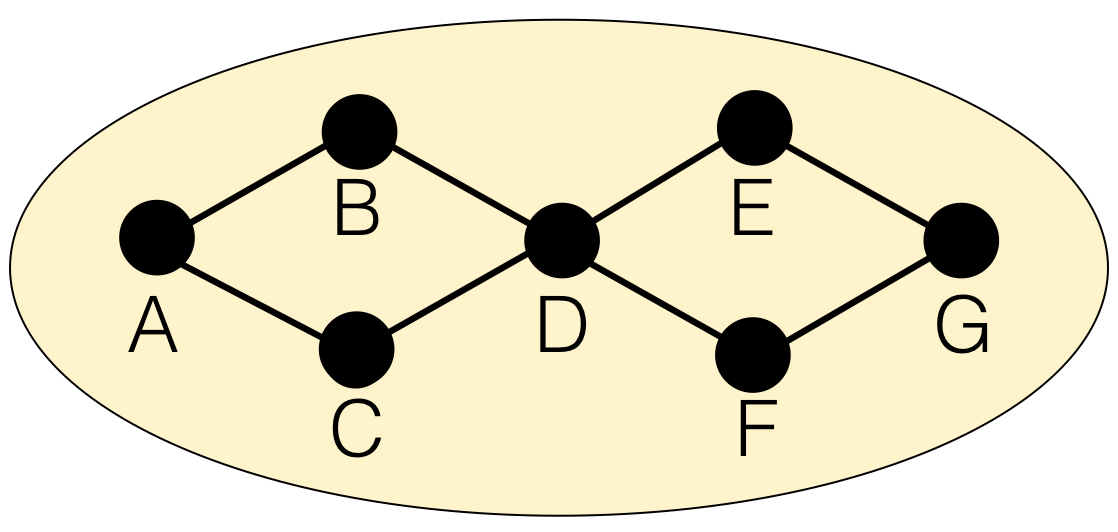
\includegraphics[width=.8\columnwidth]{figures/unimplementable}
  \caption{Example topology for which the \sysname policy: $(\CD{A} \cdot \CD{B} \cdot \CD{D} \cdot \CD{E} \cdot \CD{G}) \Prefer (\CD{A} \cdot \CD{C} \cdot \CD{D} \cdot \CD{F} \cdot \CD{G})$ is unimplementable in BGP under arbitrary failures.}
  \label{fig:unimplementable}
  %\vspace{-1em}
\end{figure}


\para{Problem Formulation}

The problem of determining local preferences for each router is closely reflected in the structure of the PGIR. In particular, whenever a given router appears in multiple different contexts in the PGIR (i.e., as multiple PGIR nodes that shadow each other), then the compiler must decide which context to prefer.
%
In our compilation example from Figure~\ref{fig:example-compilation}, the topology node $C$ can receive an advertisement from $E$ in context $(C,-,2)$ or it can receive an advertisement from its neighbor $D$ in context $(C,3,2)$.
%
The compiler's task is to determine a \emph{total ordering} of contexts for each router in the topology, which reflects the relative preference of advertisements received in each context. For example, if the compiler determines that, for router $C$, context $(C,3,2)$ is preferred to context $(C,-,2)$, written as $(C,3,2) <_{pref} (C,-,2)$, then this means that $C$ will prefer advertisements heard from $D$ (with tag $(2,2)$) over $E$ (with tag $(-,2)$). Section~\ref{sec:abgp} discusses our encoding of preferences and filters in more detail.

\para{Regret-free Preferences}

A natural question then is how the compiler should order PGIR contexts for each router in a way that is both \emph{sound} and \emph{complete} under all possible failures? To this end, we introduce the notion of \emph{regret-free} preferences, motivated by the observations from the example in Figure~\ref{fig:unimplementable}. Router $r$ has a \emph{regret-free} preference for a set of advertisements $X$ over $Y$ if, whevever $r$ selects an advertisement from $X$ over another from $Y$, there is always some policy-compliant path to each final (advertisement) destination $d$ that is at least as good $(\leq_{rank})$ as any possible path to $d$ if it had accepted an advertisement from $Y$ instead. In other words, the preference of $X$ over $Y$ at $r$ is regret-free if we are never worse off by choosing from $X$.
%
In the compilation example from Figure~\ref{fig:example-compilation}, the choice for $C$ to prefer context $(C,3,2)$ to $(C,-,2)$ is regret-free, since there will always be at least as good a path to destination $W$ regardless of any failures that might occur in the network.

%We now explain this property more formally in terms of the structure of the PGIR. We use the notation $path(s,d)$ to say that there exists a path in the PGIR from $s$ to $d$.
%
%Preferences (for the PGIR) are \emph{regret-free} if, given (i) any combination of failed topology links\footnote{Note that a single failure in the topology may correspond to zero or more failed nodes/edges in the PGIR}, (ii) a fixed topology (advertisement) destination $d$, and (iii) two contexts $N_1 < N_2$, then whever there exists a $d'$ such that $loc(d') = d$ and $path(N_2,d')$, then there exists a $d''$ such that $loc(d'') = d$ and $path(N_1,d'')$ with $d'' \leq_{rank} d'$.
%
%The property simply says that if router $N$ prefers context $N_1$ to $N_2$, then any time there is a path from $N_2$ to some destination $d$, then there exists a better (lower ranked) path from $N_1$ to destination $d$.
%



\para{A Preference Inference Algorithm}

%For example, in our compilation example from Figure~\ref{fig:example-compilation}, the topology node $C$ can receive an announcement from $E$ and later achieve the backup path, or it can receive an announcement from its neighbor $D$ and later achieve either the primary or backup path. Is it safe for $C$ to prefer its neighbor $D$ over its other neighbor $E$? The important observation is that, if $C$ prefers $D$, then it is never worse off---it will always achieve at least as good a path as if it had choosen $E$.
%For example, suppose $C$ chooses a route from $D$, but cannot achieve its primary path because the $A$ -- $W$ link has failed. In this case, the advertisement from $C$ will still be sent along towards the ultimate backup location $W$. Since the $(C,3,2)$ node has the same one-step and two-step next hops as node $(C,-,2)$ in the product graph, no possible failure will prevent a route advertisment from reaching $(W,-,4)$ that wouldn't have otherwise prevented it if $C$ had choosen $E$.

Searching for \emph{regret-free} preferences in general is hard, and enumerating all possible combinations of failures and preference orderings is intractable. We thus adopt a conservative analysis that we found to be both effective and efficient in practice. The idea is to $i)$ search for regret-free preferences by comparing the set of paths available after accepting advertisments in two different PGIR contexts $N_1$ and $N_2$, and $ii)$ refine the comparison when necessary by considering where the announcements must have traversed before arriving at $N_1$ or $N_2$.

\begin{algorithm}[t!]
\caption{Inferring regret-free preferences}
\label{alg:failures}
\begin{algorithmic}[1]
\Procedure{Regret-free($G$, $N_1$, $N_2$)}{}
  \If {$loc(N_1) \neq loc(N_2)$} \Return false
  \EndIf
  \State $q \gets Queue()$
  \State $q.Enqueue (N_1, N_2)$
  \While {$!q.Empty()$}
    \State $(n_1,n_2) \gets q.Dequeue()$
    \If {$n_1 \nleq_{rank} n_2$}
      \Return false
    \EndIf
    \For {$x$ in adj($G$, $n_2$)}
      \If {\big($\exists y \in$ adj($G$,$n_1$), shadows $x$\big) \textbf{or} \\
            \hspace{5.2em} \big($\exists y \in$ $G$, dominates $n_1$, shadows $x$\big)}
        \If {$(x,y)$ not marked}
          \State {mark $(x,y)$ as seen}
          \State $q.Enqueue(x,y)$
        \EndIf
      \Else { \Return $false$}
      \EndIf
    \EndFor
  \EndWhile
  \Return true
  \EndProcedure
\end{algorithmic}
\end{algorithm}


Algorithm~\ref{alg:failures} checks whether one context can be preferred to another ($N_1 <_{pref} N_2$). The algorithm walks from nodes $N_1$ and $N_2$ and ensures that for every \textit{step} $N_2$ can take to some new topology location, $N_1$ can, at the very least, also take a step to an equivalent topology location. When there is no such equivalent step, the algorithm attempts to take into account where the advertisement must have already traversed. In particular, it checks to see if there is an equivalent dominator (a topology location the advertisement must have passed through earlier) and walks from this new node instead.
At each step, it requires that current node reachable from $N_1$ has a path rank that is at least as good as that of the current node reachable from $N_2$ ($n_1 \leq_{rank} n_2$). The intuition here is that if $n_1 \nleq_{rank} n_2$, then we can likely fail every edge in the topology except for the path that leads to the current $n_1$ and $n_2$, thereby generating in a counter example.
Algorithm~\ref{alg:failures} terminates since the number of related states $(x,y)$ that can be explored is finite.

For each router in the topology, local preferences are now obtained by sorting the corresponding PGIR contexts according to the $(<_{pref})$ relation. If two nodes are incomparable, then the compiler rejects the policy as unimplementable.

\para{Avoiding Loops}

The checks for failure safety described above overlooked one critical point: A better (lower rank) path might not be available due to loops that are rejected by BGP. To avoid this situation, the compiler checks that, any time some context $N_1$ appears ``above'' (i.e., can reach) $N_2$ in the PGIR, then $N_1$ must be strictly preferred to $N_2$. The idea is that anytime $N_2$ is not usable because the advertisement already went through $N_1$, it ultimately does not matter since $N$ has a regret-free preference for $N_1$ anyway.


%It is fine however, to reuse the same nodes that appear above $x$, since any path that went through another node $z$ to get to $x$, but then looped through $z$ again, would be obtainable from $z$ itself.
%even if the analysis determines that a node $x$ protects against failures of another node $y$, it may be tricked into thinking $x$ has a particular path that will actually be discarded by BGP's loop prevention mechanism due to locations previously traversed before arriving at $x$. To avoid this situation, the compiler conservatively checks that $x$ protects against $y$ without using any nodes that shadow another node that appears above $x$ in the PGIR (i.e., nodes reachable from $x$ in $G_j^R$). It is fine however, to reuse the same nodes that appear above $x$, since any path that went through another node $z$ to get to $x$, but then looped through $z$ again, would be obtainable from $z$ itself.

\subsection{Aggregation-safety analysis}

%\para{Aggregation Safety}
\label{sec:agg-safety}

\begin{figure}[t!]
  \centering
  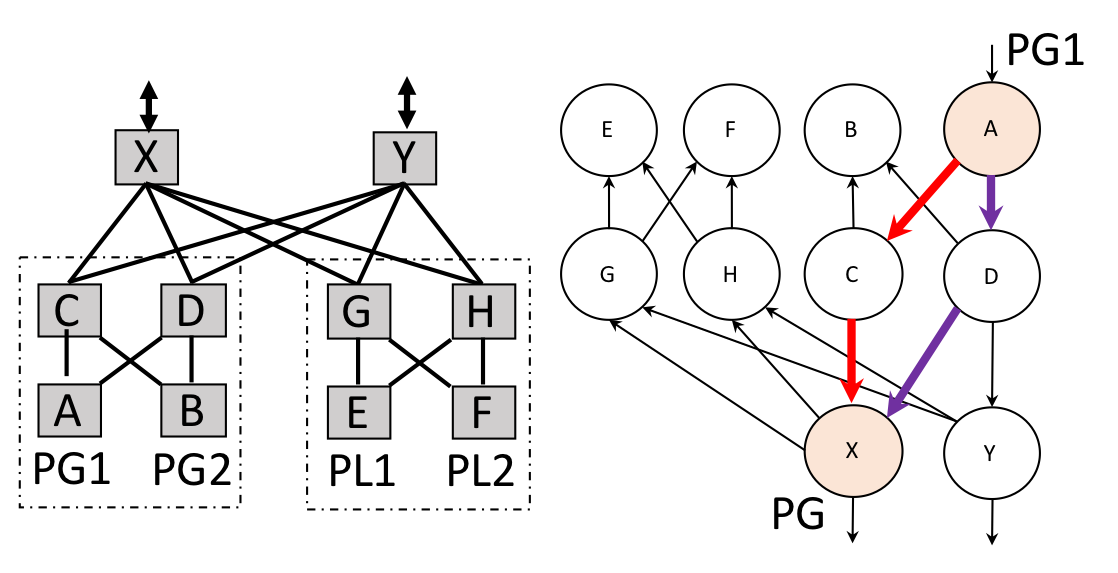
\includegraphics[width=\columnwidth]{figures/aggregation}
  \caption{Aggregation safety for a datacenter.}
  \label{fig:aggregation-safety}
  \vspace{-1em}
\end{figure}

As shown in \S\ref{sec:motivation}, BGP aggregation can lead to subtle black-holing of traffic when failures occur. Deciding when this can happen requires knowledge of the routing policy and not just the topology. For instance, a policy might require all traffic for a particular prefix to go over a single link before being aggregated, even if there are several available in the toplogy. If that link fails, a black hole might be introduced.
%
Because the PGIR encodes the complete user policy and topology,  \sysname can efficiently check that aggregates do not black hole traffic for up to $k$ failures.

We frame the aggregation problem as a problem of connectivity in the PGIR. Specifically, for each prefix that falls under an aggregate, we find a lower bound on the number of failures required to disconnect the prefix origin from its aggregation point. The difficulty is that the same links in the topology can appear in multiple places in the PGIR.
%

We adopt the following simple strategy to find a lower bound on
the number of failures: $i)$ pick a random start-to-end path in the PGIR, $ii)$ remove all edges in the PGIR for the set of topological edges chosen, and $iii)$ repeat until no such path exists.
The number of PGIR paths that we are able to remove is a lower bound on the number of failures required to disconnect the prefix from its aggregate.

For example, recall the datacenter example from \S\ref{sec:motivation}, with the policy
\CD{PG1} \Path \text{ }\End(\CD{A}), where \CD{PG1} falls under the \CD{PG} aggregate. Figure~\ref{fig:aggregation-safety} shows the simplified PGIR. Since the compiler knows aggregation will occur at $X$, and it knows that the \CD{PG1} prefix will originate at $A$, we can compute the number of failures it would take to disconnect $A$ from $X$. We could remove the $A$--$D$--$X$ path first. We would then need to remove any other $A$--$D$ or $D$--$X$ links from the PGIR (in this case none). Next, we could remove the links along the $A$--$C$--$X$ path, repeating the process. Because $A$ is then disconnected from $X$, the compiler knowns that 2 is a lower bound on the number of failures for aggregation safety for prefix \CD{PG1}. This process is repeated for other aggregation locations (e.g., $Y$).


\subsection{Abstract BGP}
\label{sec:abgp}


%\begin{figure}[t!]
%\centering
%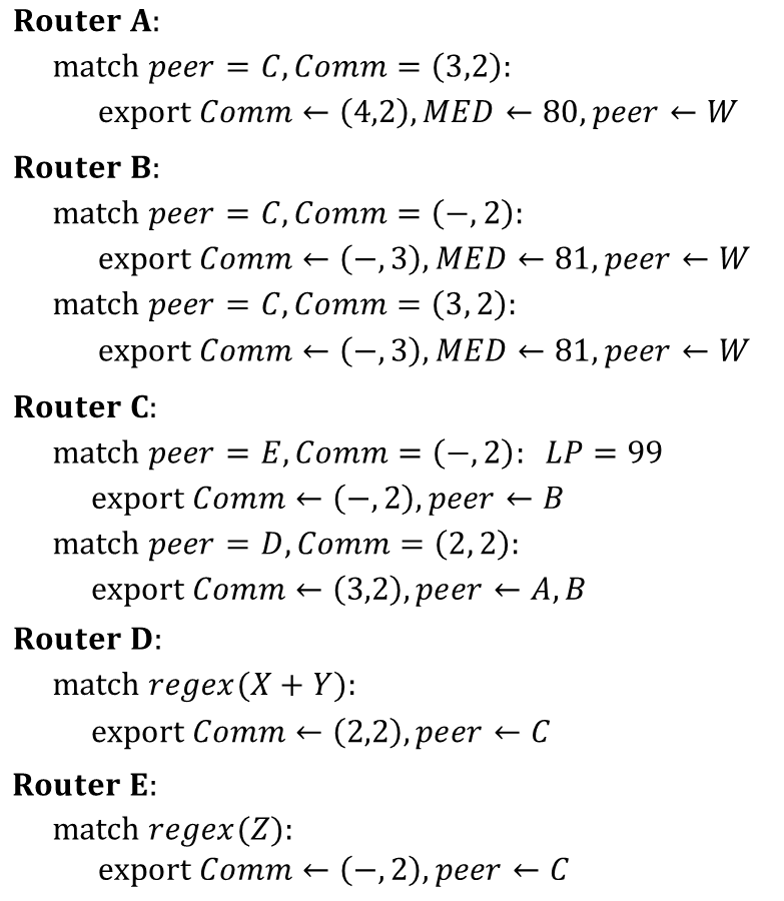
\includegraphics[width=.9\columnwidth]{figures/config}
%\caption{Abstract BGP configuration.}
%\label{fig:abgp-config}
%\end{figure}

\newcommand{\highlight}[1]{%
  \colorbox{red!50}{$\displaystyle#1$}}
\newcommand{\Router}[1]{\KW{Router} #1:}
\newcommand{\REGEX}[1]{\texttt{regex}(#1)}
\newcommand{\PEER}{\texttt{peer}}
\newcommand{\COMM}{\texttt{comm}}
\newcommand{\MED}{\texttt{MED}}
\newcommand{\Arrow}{\ensuremath{\leftarrow}}



%\begin{figure}[t!]
%\begin{lstlisting}[frame=single, mathescape=true]
%$\Router{A}$
%  Match $\PEER=C$
%    Export $\MED \leftarrow 80, \PEER \leftarrow W$
%$\Router{B}$
%  Match $\PEER = C$
%    Export $\COMM \leftarrow \text{noexport}, \MED \leftarrow 81, \PEER \leftarrow W$
%$\Router{C}$
%  Match$[LP=99]$ $\PEER = E $
%    Export $\PEER \leftarrow B$
%  Match $\PEER = D$
%    Export $\PEER \leftarrow A,B$
%$\Router{D}$
%  Match $\REGEX{X + Y}$
%    Export $\PEER \leftarrow C$
%$\Router{E}$
%  Match $\REGEX{Z}$
%    Export $\PEER \leftarrow C$
%\end{lstlisting}
%\label{fig:config-min}
%\caption{Abstract BGP minimized configurations}
%\end{figure}

The final stage of our compiler translates policies from PGIR to a vendor-neutral abstraction of BGP (ABGP).
% and then from ABGP to actual device configurations.

\begin{figure}[t!]
\begin{code}
  \Router{A}
    Match \PEER=C, \COMM=(3,2)
      Export \COMM \Arrow (4,2),
             \MED \Arrow 80, \PEER \Arrow W
  \Router{B}
    Match \PEER = C, \COMM = (-,2)
      Export \COMM \Arrow (-,3), \COMM \Arrow \text{noexport},
             \MED \Arrow 81, \PEER \Arrow W
    Match \PEER = C, \COMM = (3,2)
      Export \COMM \Arrow (-,3), \COMM \Arrow \text{noexport},
             \MED \Arrow 81, \PEER \Arrow W
  \Router{C}
    Match[LP=99] \PEER = E, \COMM = (-,2)
      Export \COMM \Arrow (-,2), \PEER \Arrow B
    Match \PEER = D, \COMM = (2,2)
      Export \COMM \Arrow (3,2), \PEER \Arrow A,B
  \Router{D}
    Match \REGEX{X + Y}
      Export \COMM \Arrow (2,2), \PEER \Arrow C
  \Router{E}
    Match \REGEX{Z}
      Export \COMM \Arrow (-,2), \PEER \Arrow C
  \end{code}
  \vspace{-2em}
  \caption{Abstract BGP router configurations. \label{fig:abgp-config}}
  \vspace{-1em}
\end{figure}

\para{From PGIR to ABGP}

Once we have the ordering on node preferences in the PGIR from the failure safety analysis, the translation to ABGP is straightforward. The idea is to encode the state of the automata using BGP community values. Each router will match based on its peer and a community value corresponding to the state of the PGIR, and then update the state before exporting to the neighbors permitted by the PGIR. For example, router $A$ in Figure~\ref{fig:example-compilation} will allow an announcement from $C$ with a community value for state $(3,2)$ (and deny anything else). If it sees such an announcement, it will remove the old community value, and add a new one for state $(4,2)$ before exporting it to $W$.

To ensure preferred paths are always obtained, for each router $r$ in the topology, the compiler sets a higher local preference for neighbors of a more-preferred node for $r$ in the PGIR. For example, $C$ will prefer an advertisement from $D$ in state $(2,2)$ over an advertisement from $E$ in state $(-,2)$.

Since the compiler can control community tagging only for routers under the control of the AS being programmed, it cannot match on communities for external ASes. Instead, it translates matches from external ASes into a BGP regular expression filter. For example, node $D$ in Figure~\ref{fig:example-compilation} would match the single hop external paths $X$ or $Y$. In general, if routes are allowed from beyond $X$ or $Y$, these will also be captured in the BGP regular expression filters. The unknown AS topology is modelled as a special node in the PGIR that generates a filter to match any sequence of ASes.

Finally, the external AS $W$ should prefer our internal router $A$ over $B$. In general, it is not possible to reliably control traffic entering the network beyond certain special cases. In this example, however, assuming our network and $W$ have an agreement to honor MEDs, the MED attribute can influence $W$ to prefer $A$ over $B$. Additionally, the compiler can use the BGP no-export community to ensure that no other AS beyond $W$ can send us traffic. The compiler can perform a simple analysis to determine when it can utilize BGP special attributes to ensure traffic enters the network in a particular way by looking at links in the product graph that cross from the internal topology to the external topology.
%Aggregation is another tool commonly used to influence how traffic can enter the network, by relying on BGP's longest prefix matching default. Since aggregates are provided as additional user constraints, the compiler can also make use of this information to check that incoming preferences can be met given the aggregates specified (e.g., to ensure that all external ASes prefer to enter from one location over another).
Figure~\ref{fig:abgp-config} shows the full configuration from the compilation example.

After configuration generation, the compiler further processes the ABGP policy, removing community tags when possible, combining filters, removing dead filters, and so on. In the compilation example, all community tags can be removed since there is never any ambiguity based on the router importing the route, and the neigbor the route is being imported from. Similarly, after removing the communities, the two rules at router $B$ are merged into a single rule.


%=====================================================
%
%
%  **Implementation**
%
%
%=====================================================

\section{Implementation}
\label{sec:implementation}

Our \sysname compiler is implemented in roughly 6700 lines of F\# code. It includes command-line flags for enabling or disabling the use of the BGP MED attribute, AS path prepending, the no-export community, as well as for ensuring at least k-failure safety for aggregate prefixes. Since each prefix has a separate routing policy, we compile each routing policy in parallel. Currently, \sysname supports generating Quagga router configurations out of the box. Users can add new vendor-specific adaptors to translate from ABGP to other router configuration languages, or incorporate the compiler into an existing template-based system, e.g., by mixing the \sysname-generated BGP configuration with other, non-BGP configuration elements.

Our compiler includes the following features that improve its performance and usability.

\para{Efficient PGIR construction}

Constructing automata for extended regular expressions (i.e., those that include negation and intersection) are known to have high complexity~\cite{regex-complexity}. The \sysname compiler uses regular expressions derivatives~\cite{regex-derivatives} with character classes to construct deterministic automata for extended regular expressions over large alphabets efficiently. Since regular expressions are defined over a finite alphabet, and since much of the AS topology is unknown, we set the alphabet to include all uniquely referenced external ASes in the policy. Similarly, to model the unknown external AS topology beyond immediate peers, we include a special topology node to represent any unknown location.
%
Rather than construct the product graph in full, our implementation prevents exploring parts of the graph when no accepting state is reachable in any of the corresponding regular automata during construction.

%\para{PG Minimization}

%The \sysname compiler uses a fast algorithm for computing graph dominators by storing sets of dominators in a compact representation known as a dominator tree~\cite{fast-dominance}. More complex algorithms with better theoretical complexity exist~\cite{linear-dominance, tarjan-dominance} and may be better suited for large enough topologies. All minimization steps are repeated until no more progress can be made.

\para{Fast failure-safety analysis}

When computing local preferences and ensuring failure safety, as described in \S\ref{sec:compilation}, the compiler performs memoization of the \textup{Regret-Free} function. That is, whenever for two states $N_1$ and $N_2$ we compute $\textup{Regret-Free}(G, N_1, N_2)$, if the function evaluates to $true$, then each of the intermediate related states $x$ and $y$ must also satisfy $\textup{Regret-Free}(G, x, y)$. Memoizing these states dramatically reduces the amount of work performed to find preferences in the common case.

\para{Efficient configuration generation}

The naive code generation algorithm described in \S\ref{sec:compilation} is extremely memory inefficient since it generates a separate match-export pair for every unique in edge/out edge pair for every node in the product graph before minimization. Our implementation performs partial minimization during generation by recognizing common cases such as when there is no restriction on exporting to or importing from neighbors.


\para{Checking policy correctness}

Even when programming the network centrally, it is possible for operators to make mistakes and write incorrect policies.
\sysname includes many analyses to flag common mistakes at compile time. A subset includes: (i) a preference analysis to determine when backup paths/preferences will never be used, (ii) a reachability analysis to check if topology locations that should be reachable according to the operator policy are not reachable after combining both the topology and policy, (iii) an anycast analysis to find instances where the operator accidentally anycasts a prefix (i.e., originates it from multiple locations), (iv) an aggregate analysis to find when aggregates do not summarize any specific prefix.




%=====================================================
%
%
%  **Evaluation**
%
%
%=====================================================


\section{Evaluation}
\label{sec:evaluation}


We apply \sysname on real policies for backbone and datacenter networks. Our main goals are to evaluate if its language is expressive enough for real-world policies and the time the compiler takes to generate router configurations.

\subsection{Networks studied}

We obtained routing policy for the backbone network and for the datacenters of a large cloud provider. Multiple datacenters share this policy. The backbone network connects to the datacenters and also has many external BGP neighbors. The high-level policies of these networks are captured in an English document which guides operators when writing configuration templates for datacenter routers or actual configurations for the backbone network (where templates are not used because the network has less regular structure).

The networks have the types of policies that we outlined earlier (\S\ref{sec:motivation}). The backbone network classifies external neighbors into several different categories and prefers paths through them in order. It does not want to provide transit among certain types of neighbors. For some neighbors, it prefers some links over the others. It supports communities based on which it will not announce certain routes externally or announce them only within a geographic region (e.g., West Coast of the USA). Finally, it has many filters, e.g., to prevent bogons (private address space) from external neighbors, prevent customers from providing transit to other large networks, prevent traversing providers through peers, etc.

Routers in the datacenter network run BGP using private AS numbers and peer with each other and with the backbone network over eBGP. The routers aggregate some prefix blocks when announcing them to the backbone network, they keep some prefixes internal, and attach communities for some other prefixes that should not traverse beyond the geographic region. The datacenter networks also have policies by which some prefixes should not be announced beyond a certain tier in the datacenter hierarchy.

\begin{figure}
  \subcaptionbox{Datacenter}
    {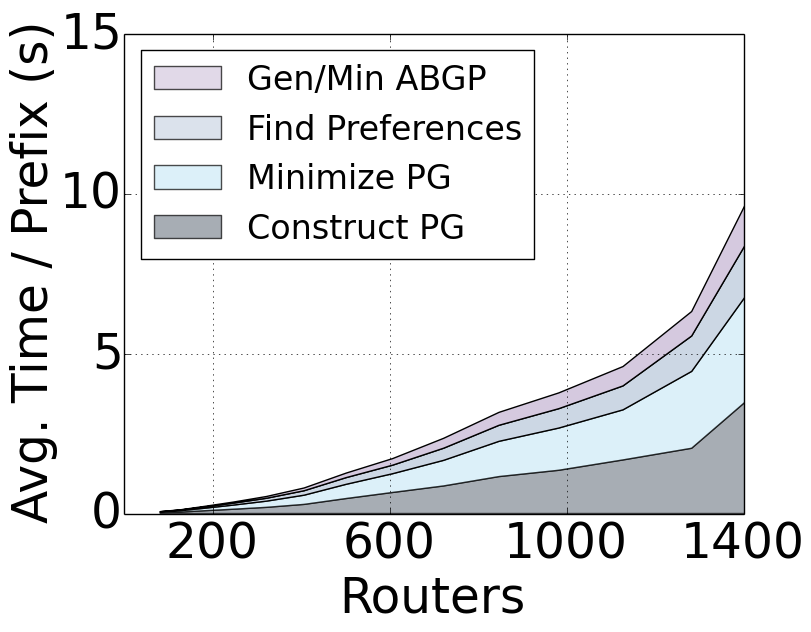
\includegraphics[width=.49\columnwidth]{figures/compilation-times-dc.png}}
  \subcaptionbox{Backbone}
    {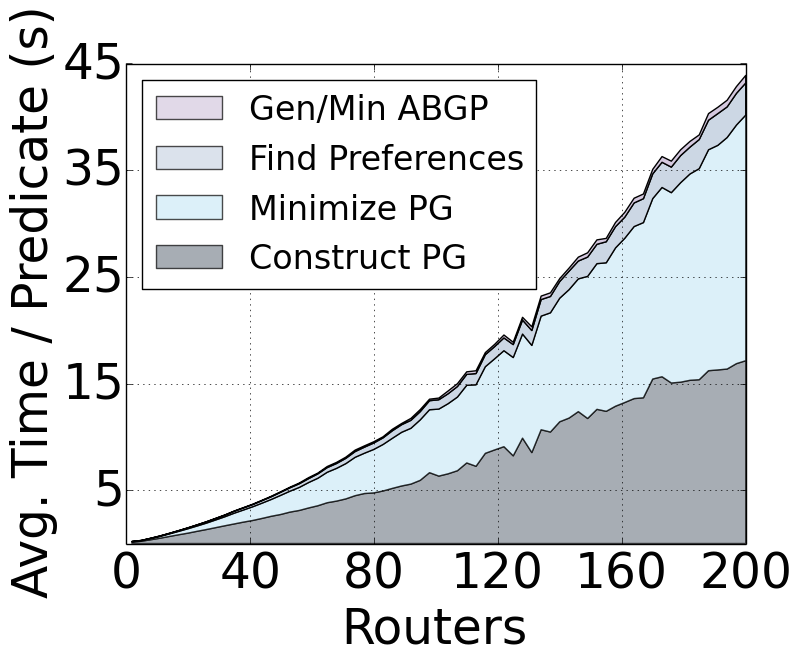
\includegraphics[width=.49\columnwidth]{figures/compilation-times-backbone.png}} \\
  \caption{Compilation time. \label{fig:compilation-times}}
  \vspace{-1em}
\end{figure}


\subsection{Expressiveness}

We found that we could translate all network policies to \sysname. We verified with the operators that our translation preserved intended semantics.\footnote{Not intended as a scientific test, but we also asked the two operators if they would find it easy to express their policies in \sysname. The datacenter operator said that he found the language intuitive. The backbone operator said that formalizing the policy in \sysname seemed equally easy or difficult as formalizing in RPSL~\cite{RFC2622}, but he appreciated that he would have to do it only once for the whole network (not per-router) and did not have to manually compute various local preferences, import-export filters, and MEDs.} We found that the datacenter policies were correctly translated. For the backbone network, the operator mentioned an additional policy that was not present in the English document, which we added later.

Not counting the lines for various definitions like prefix and customer groups or for prefix ownership constraints, which we cannot reveal because of confidentiality concerns, the routing policies for \sysname were 43 lines for the backbone network and 31 lines for the datacenter networks.


\subsection{Compilation time}


%\begin{figure}[t!]
%  \centering
%  \begin{minipage}[b]{0.45\linewidth}
%    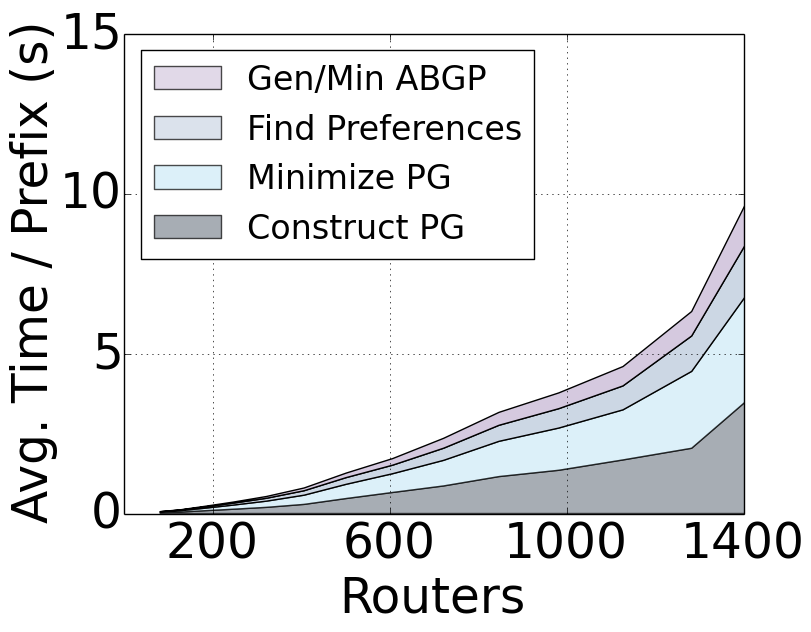
\includegraphics[width=1.1\columnwidth]{figures/compilation-times-dc.png}
%  \end{minipage}
%  \quad
%  \begin{minipage}[b]{0.45\linewidth}
%    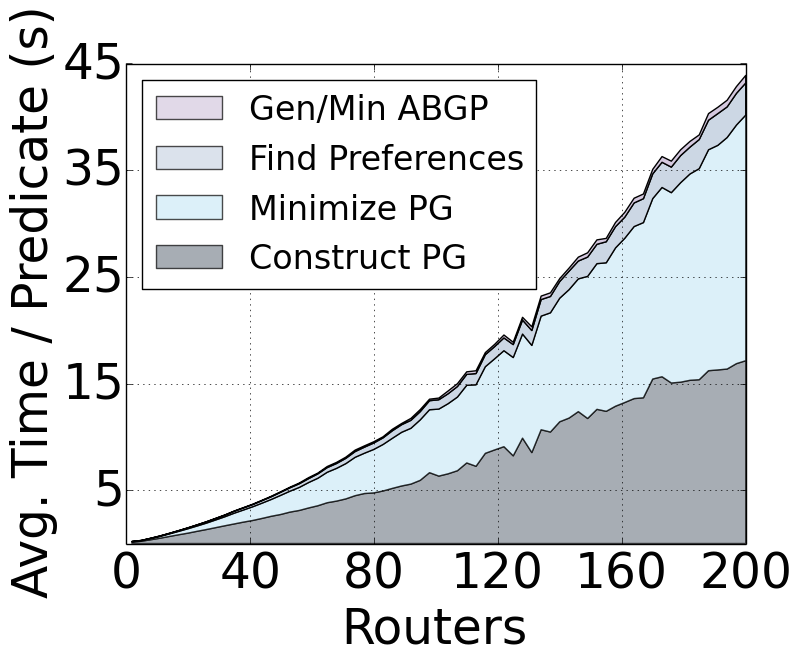
\includegraphics[width=1.1\columnwidth]{figures/compilation-times-backbone.png}
%  \end{minipage}
%  \caption{Compilation times.}
%  \label{fig:compilation-times}
%\end{figure}

%\begin{figure}[t!]
%  \centering
%  \begin{minipage}[b]{0.45\linewidth}
%    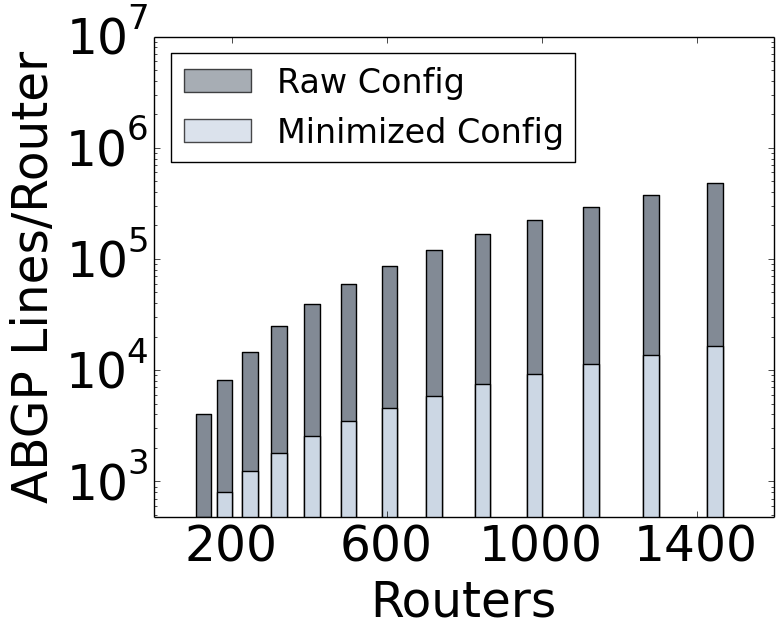
\includegraphics[width=1.1\columnwidth]{figures/config-compression-dc.png}
%  \end{minipage}
%  \quad
%  \begin{minipage}[b]{0.45\linewidth}
%    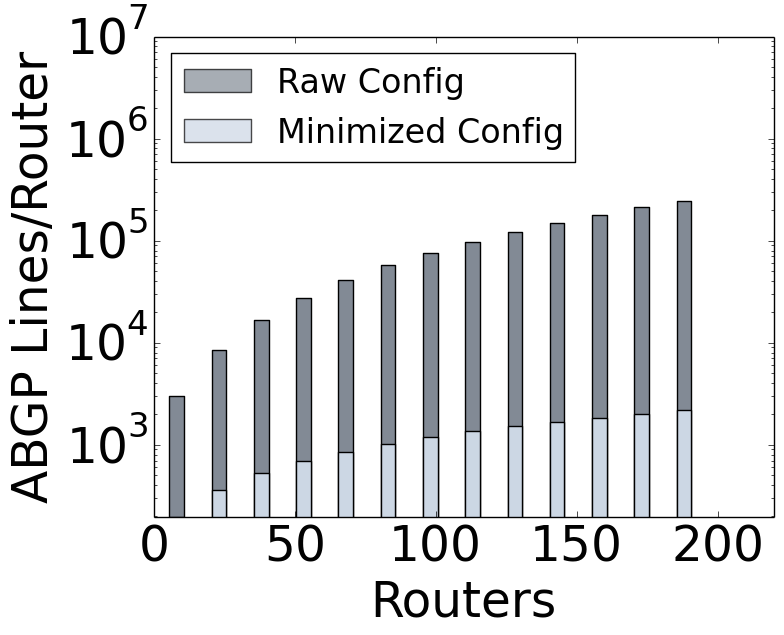
\includegraphics[width=1.1\columnwidth]{figures/config-compression-backbone.png}
%  \end{minipage}
%  \caption{Configuration minimization.}
%  \label{fig:config-minimization}
%\end{figure}

We study the compilation of time for both policies as a function of network size. Even though the networks we study have a fixed topology and size, we can explore the impact of size because the policies are network-wide and the compiler takes topology itself as an input. For the datacenter network, we build and provide as input fat tree~\cite{fattree} topologies of different sizes, assign a /24 prefix to each ToR switch, and randomly map prefixes to each type of prefix group with a distinct routing policy.
%We take this approach to smoothly explore different sizes.
%There is a parameterized way to build fat trees~\cite{fattree}, which does not exist for our concrete datacenter topologies. For a given size, our reported results match those for the concrete topologies.
For the backbone network, the internal topology does not matter since all routers connect to each other through iBGP. We explore different (full iBGP) mesh sizes and randomly map neighboring networks to routers. Even though each border router connects to many external peers, we count only the mesh size.

All experiments are run on an 8 core, 3.6 GHz Intel Xeon processor running Windows 7.
%
Figure~\ref{fig:compilation-times} shows the compilation times for datacenter and backbone networks of different sizes. For both policies, we measure the mean compilation time per prefix predicate since the compiler operates on predicates in parallel. A single predicate can describe many prefixes, for example by matching on a disjunction of prefixes. At their largest sizes, the per-predicate compilation time is roughly 10 seconds for the datacenter network and 45 seconds for the backbone network.

%From the break down of the time by compilation phase, we see that no single compilation phase dominates the running time of the compiler. However, construction and minimization of the product graph take the most time.

Total compilation for the largest datacenter is less than 9 minutes total. Unlike the datacenter policy, the number of prefixes for the backbone policy remains relatively fixed as the topology size increases. Compilation for the largest backbone network, takes less than 3 minutes total. The inclusion of more preferences in the backbone policy increases the size of the PGIR, which leads to PGIR construction and minimization taking proportionally more time.

In both examples, we observe that our failure-safety analysis algorithm for finding preferences is highly efficient, taking only a small fraction of the total running time. PGIR minimization is the most expensive compilation phase. If needed, minimization can be capped after a certain number of iterations for large networks. Both the backbone and datacenter  policies we considered can be successfully compiled without minimization.

%

\begin{figure}[t!]
  \subcaptionbox{Datacenter}
    {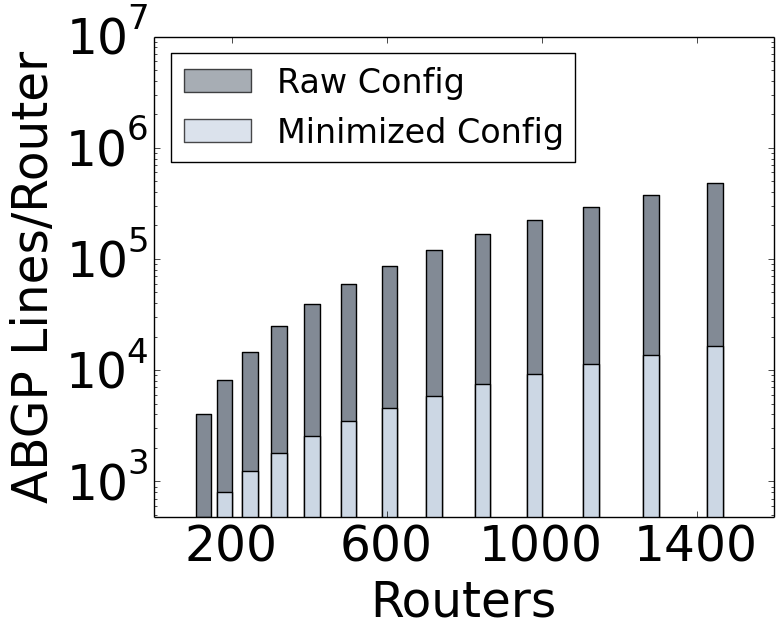
\includegraphics[width=.49\columnwidth]{figures/config-compression-dc.png}}
  \subcaptionbox{Backbone}
    {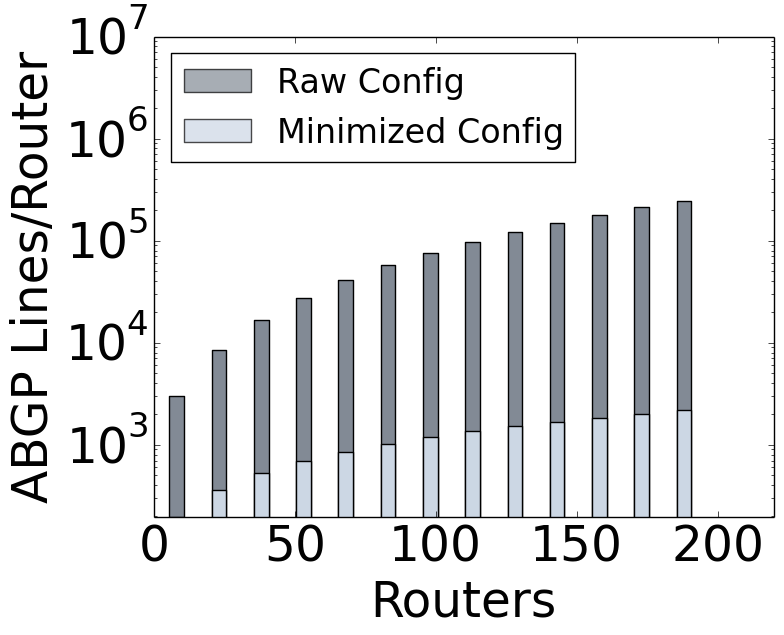
\includegraphics[width=.49\columnwidth]{figures/config-compression-backbone.png}} \\
  \caption{Configuration minimization. \label{fig:config-min}}
  \vspace{-1em}
\end{figure}

\subsection{Configuration size}

Figure~\ref{fig:config-min} shows the size of the compiled ABGP policies as a function of the topology size. The naive translation of PGIR to ABGP outlined in \S\ref{sec:compilation} generates extremely large ABGP policies by default. To offset this, the compiler performs ABGP configuration minimization both during and after the PGIR to ABGP translation phase.
%Such minimization is useful for limiting the computational expense of matching routes on BGP routers, reducing the number of forwarding entries in routers in certain cases, and making configurations more readable for humans.
Minimization is highly effective for both the datacenter and backbone policies. In all cases, minimized policies are a small fraction of the size of their non-minimized counterparts.

%for i in *.set; do grep bgp $i | wc; done
However, even minimized configurations are hundreds or thousands of lines per router. For the backbone network, the size of \sysname configurations is roughly similar to the BGP components of actual router configurations, though qualitative differences exist (see below). We did not have actual configurations for the datacenter network; they are dynamically generated from templates.


\subsection{Propane vs. operator configurations}

We comment briefly on how \sysname-generated configurations differ from configurations or templates generated by operators.
%
In some ways, \sysname configurations are similar. For example, preferences among neighboring ASes are implemented with a community value to tag incoming routes according to preference, which is then used at other border routers to influence decisions.

In other ways, the \sysname configurations are different, relying on a different BGP mechanism to achieve the same result. Some key differences that we observed were:

$i)$ operators used the no-export community to prevent routes from leaking beyond a certain tier of the datacenter, while \sysname selectively imported the route only below the tier;
%\sysname could use a similar implementation mechanism in the future as an optimization.

$ii)$ operators prevented unneeded propagation of more-specific route announcements from a less-preferred neighboring AS based on their out-of-band knowledge about the topology, whereas \sysname propagated these advertisements;

$iii)$ operators used a layer of indirection for community values, using community groups and re-writing values, to implement certain policies in a more maintainable manner, where \sysname uses flat communities; and

$iv)$ operators used BGP regular expression filters to enforce certain invariants that are independent of any particular prefix, whereas \sysname enforced these invariants per prefix.

We are investigating if such differences matter to operators, e.g., if they want to read \sysname configurations, and, if necessary, how to reduce them.




%=====================================================
%
%
%  **Related Work**
%
%
%=====================================================

\section{Related Work}
\label{sec:related}

Our work draws on four threads of prior work.

\para{SDN languages}
\sysname{} was heavily influenced by SDN programming
languages such as NetKAT~\cite{netkat}, Merlin~\cite{foster:merlin}, FatTire~\cite{fattire},
as well as path queries~\cite{queries}.
Each of these languages is oriented around regular expressions, which
describe paths through a network, and predicates, which classify packets.
In particular, FatTire allows programmers to define sets of paths together
with a fault tolerance level (\emph{i.e.,} tolerate 1 or 2 faults)
and the compiler generates appropriate OpenFlow rules.
\sysname is more expressive as it allows users to specify preferences among
paths, and it generates distributed implementations that tolerate any number of faults.
Because FatTire generates data plane rules up front,
specifying higher levels of fault tolerance comes
at the cost of generating additional rules that tax switch memory.
In contrast, \sysname relies on distributed
control plane mechanisms to react to faults, which do not have additional memory cost.
Because of the differences in the underlying technology, the analyses
and compilation algorithms used in \sysname are quite different from
previous work on SDN.
Finally, in addition to using path-based abstractions
for intra-domain routing, \sysname uses them for inter-domain routing as
well, unlike existing SDN languages.

\para{Configuration automation}
Many practitioners use configuration templates~\cite{hatch,thwack}, to ensure certain kinds of consistency across similar devices. In addition, configuration languages such as RPSL~\cite{RFC2622}, Yang~\cite{RFC6020}, and Netconf~\cite{RFC6241} allow operators to express routing policy in a vendor-neutral way.
However, all of these solutions remain low-level, for example, requiring operators to specify exact local preferences. Unlike \sysname, there is no guarantee that these low-level configurations satisfy the original, high-level intent.

\para{Configuration analysis}
The notion that configuring network devices is difficult and error-prone is not new.
In the past, researchers have tried to tackle this problem by analyzing existing
firewall configurations~\cite{fang,lumeta,margrave} and
router configurations~\cite{feamster+:rcc,feamster:thesis,ipassure,batfish,bagpipe,arc} and reporting errors or inconsistencies when they are detected.
Our research is complementary to these analysis
efforts.  We hope to eliminate bugs by using higher-level
languages and a ``correct-by-construction''
methodology.  By proposing network administrators write configurations
at a high-level of abstraction, a whole host of low-level errors can be avoided and policy implementation can be simplified.

\para{Configuration synthesis}
ConfigAssure~\cite{narain:lisa05,narain+:configassure}
is another system designed to
help users define and debug low-level router
configurations.  Inputs to
ConfigAssure include a \emph{configuration database}, which contains a
collection of tuples over constants and configuration variables, and a
\emph{requirement}, which is a set of constraints.
%For instance, the tuple \texttt{hsrp(rexa,rA1,int(1),int(2))} states that interface
%\texttt{rA1} on device \texttt{rexa} belongs to the HSRP group defined
%by configuration variable \texttt{int(1)} with virtual IP address
%defined by configuration variable \texttt{int(2)}.  The constraint
%\texttt{hsrp\_subnet([rexa-rA1,rexb-rB1])} states that a database
%contains tuples defining HSRP group identifiers and virtual IPs for
%interfaces \texttt{rA1} and \texttt{rB1} on devices \texttt{rexa} and
%\texttt{rexb}.
The authors use a combination of logic programming and
SAT solving to find concrete values for configuration variables.
%such as \texttt{int(1)}.
ConfigAssure handles configuration for a wide range of protocols and many
different concerns.  In contrast, the scope of \sysname is much
narrower.  In return, \sysname offers compact, higher-level
abstractions customized for our domain, such as regular paths, as well
as domain-specific analyses customized to those abstractions, such as
our failure safety analysis.  The implementation technology is also
entirely different, as we define algorithms over automata and graphs
as opposed to using logic programming and SAT-based model-finding.

%We also believe the high-level, centralized nature of \sysname policies
%has the benefit of making configurations
%easier to understand and maintain.



%=====================================================
%
%
%  **Future Work**
%
%
%=====================================================


%\section{Future Work}
%
%There are a number of possible directions for future work in programming distributed control planes. One option would be to integrate a model of the environment into the compiler. For example, many ASes make use of informal peering agreements (e.g., tagging routes with certain communities) to enable a wider range of policies. A compiler with this information, could automatically derive routes conforming to these agreements.
%
%Another direction would be to perform policy verification at the level of centralized language. There has been great deal of work on verification of the data plane, but much less so on control plane verification. The \sysname language provides a high-level abstraction of the control plane, which could be amenable to verification or checking equivalence of policies. For example, an operator could check if adding aggregation at various points in the network as an optimization ever changes routing behavior. The automata-based representation of the product graph may lend itself well to this kinds of analysis.
%
%While we target BGP in this paper as a distributed backend for \sysname due to its expressiveness, scalability, and uniformity, it should be possible to use other protocols to achieve different types of routing policies (e.g., OSPF). In particular, one could potentially combine different distributed routing protocols through route redistribution to achieve a larger variety of policies.
%
%Another possible future direction is automate AS-wide load balancing for BGP. Load-balancing with BGP across external ASes is difficult since there are few mechanisms at the operators disposal. However BGP policies can artificially prepend to the AS path to increases its length, and influence peer decisions. The product graph representation describes, not only which neighbors routers should prefer, but also which neighbors it is indifferent towards. Thus the compiler knowns when it can safely perform load-balancing across different neighbors.




%=====================================================
%
%
%  **Conclusions**
%
%
%=====================================================

\section{Conclusions}
\label{sec:conclusions}

We introduced \sysname, a language and compiler for implementing network-wide policies using a distributed set of devices running BGP. Propane allows operators to describe their policy naturally through high-level constraints on the shape and relative preferences of paths for different types of traffic. When \sysname compiles a policy, the resulting BGP configurations are correct-by-construction and faithfully implement the policy in a distributed fashion, regardless of the number and combinations of failures. Applying \sysname to real-world networks showed that its language is expressive and its compiler is scalable. 



%=====================================================
%
%
%  **Appendix**
%
%
%=====================================================


%\subsection{Propane Properties}
%
%\newtheorem{prop}{Proposition}[section]
%
%Here we investigate the correctness and expressiveness properties of \sysname. We are mainly concerned with answering the following questions: (1) does the distributed, compiled policy faithfully implement the user's policy regardless of failures? (2) Are the resulting BGP configurations stable?, and (3) what polcies are or are not expressible in \sysname?
%
%If \sysname compiles a user policy to a distributed implementation, then that distributed implementation faithfully meets the centralized policy's semantics under any failure scenario. We are primarily concerned with the steady state: that is, what happens after (if) the routing protocol converges. We argue that \sysname is correct by breaking down the claim:
%
%\begin{prop}
%BGP configurations for internal routers produced by \sysname will be stable.
%\end{prop}
%
%\begin{prop}
%BGP configurations produced by \sysname are \textit{Sound} with respect to the policy: That is, any route traffic takes in the network, is a valid route specified by the policy.
%\end{prop}
%
%The Soundness claim follows directly from compilation of the product graph. Since every path through the product graph (from start to end) must match the user's policy, and since the compiled configurations use communities to ensure only valid routes through the product graph are used, the resulting BGP configurations are Sound.
%
%\begin{prop}
%BGP configurations produced by \sysname are \textit{Complete}: That is, the distributed implementation always obtains a most preferred route between two nodes when the corresponding path exists in the network.
%\end{prop}
%
%The argument for completeness is as follows: Assume the most preferred path that exists in the network is between two nodes $X$ and $Y$.  This means there is a valid path in the product graph corresponding to this path, and which is available in the network.
%Assume we are unable to achieve this route in the network. To not achieve this path means that some router along the advertisement route from $Y$ to $X$ preferred to accept an advertisement from another peer instead. This implies that router that makes the ``wrong'' choice appears as a separate node in the product graph. However, from our failure safety check, we know that the other, more-preferred node must have a superset of the paths to accepting states as the less preferred node (from which it stole the route) for at least as good of a final preference. The argument then proceeds by induction on the path length - there are only a finite number of such stealings that can occur, each of which will ultimately still result in a route advertisement reaching $X$ along a most preferred path.
%
%Any \sysname-compiled policy will be \textit{Complete} as a result of the failure safety check.
%

%

%The combination of Soundness and Completeness ensures that the distributed implementation will always send traffic along the best paths possible, yet will also never also use any undesired paths. These properties rely on the fact that \sysname produces stable BGP configurations:

%
%The reduction is via the well-known No-Dispute-Wheel condition~\ref{bib:todo} for stable BGP. In particular, any policy with a dispute wheel will not pass the stronger failure safety check by \sysname.
%
%\begin{figure}[t!]
%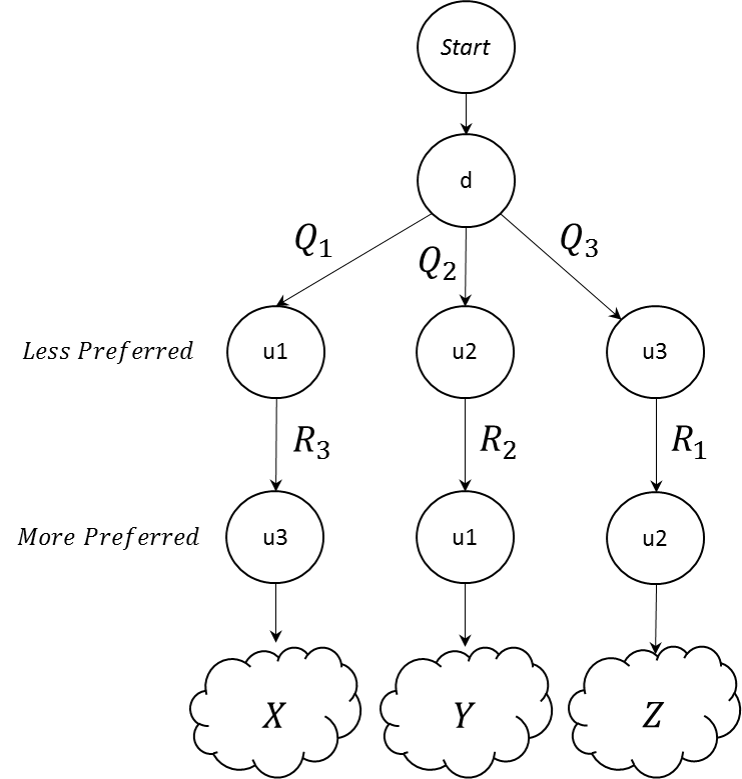
\includegraphics[width=\columnwidth]{figures/dispute-wheel}
%\label{fig:dispute-wheel}
%\caption{Product graph for a dispute wheel.}
%\end{figure}
%
%The reduction is via the well-known No-Dispute-Wheel condition~\ref{bib:todo}. If a set of BGP configurations do not have a dispute wheel, then they will converge to their best routes. Any BGP policy with a dispute wheel will not satisfy the failure safety condition in Section~\ref{sec:compilation}. Assume that the preferences in the policy describe a dispute wheel, and we will show that our failure check will reject the policy. Informally, a dispute wheel occurs when there are some number of nodes $u_1, \dots, u_n$ attempting to get a path to a destination node $d$. Each node $u_i$ prefers to go through its neighbor $u_{i+1}$ over route $R_i$ than directly to $d$ with route $Q_i$. Thus the nodes form a wheel of preferences. The product graph for a policy that contains a dispute wheel will look like Figure~\ref{fig:dispute-wheel}, which shows a dispute wheel of size 3. In order to pass the failure safety check for the compiler, the more-preferred node for $u_2$ will need to have a superset of the paths starting from the less-preferred node for $u_2$. In turn, this means that the maximum length path after visiting the more preferred $u_2$ will be $max(Z) = 1 + max(Y)$, similarly, if we look at $u_1$, we will determine that $max(Y) = 1 + max(X)$, and so on. The resulting equations define a system of unsatisfiable equations. Therefore, it is not possible for \sysname to compile a BGP policy that contains a dispute wheel. Since no-dispute-wheel is a sufficient condition for BGP stability, any compiled \sysname policy will be stable.
%

%An important distinction is that BGP might still be instable with respect to other external ASes, since \sysname has no way of configuring their routing policy and can only rely on AS path filters to see what advertisements are observed.




%=====================================================
%
%
%  **Bibliography**
%
%
%=====================================================

\bibliographystyle{abbrv}
\bibliography{references}

% The bibliography should be embedded for final submission.


\end{document}
